\documentclass{article}
\usepackage[utf8]{inputenc}

\title{Inteligencia Artifical Avansada para la Ciencia de Datos I}
\author{Álvaro Morán Errejón 		     | A01638034\\Héctor Manuel Cárdenas Yáñez	 | A01634615\\Isaí Ambrocio				     | A01625101\\Siddhartha López Valenzuela      | A00227694}


\date{September 4th, 2023}

\usepackage{natbib}
\usepackage{graphicx}

\begin{document}

\maketitle

\section{Introduction}
This report intends to show a solution the problem of "Activivty Recognition in Senior Citizens".  The Human Activity Recognition 70+ (HAR70+) dataset is a professionally-annotated dataset containing 18 fit-to-frail older-adult subjects (70-95 years old) wearing two 3-axial accelerometers for around 40 minutes during a semi-structured free-living protocol. The sensors were attached to the right thigh and lower back
Each subject's recordings are provided in a separate .csv file. The purpose was to train machine learning models for human activity recognition on professionally-annotated accelerometer data of fit-to-frail older adults.

\section{Libraries}
A list of all the libraries used to perform this activity are shown in the image below:

\section{Data Analysis}
    \subsection{Loading Data}

    For staters, all the data was uploaded to Google Colab and was roughly concatenated into a huge DataFrame containing 
    all the information so that it could be used for further analysis. \pagebreak
    \begin{figure}[h]
        \centering
        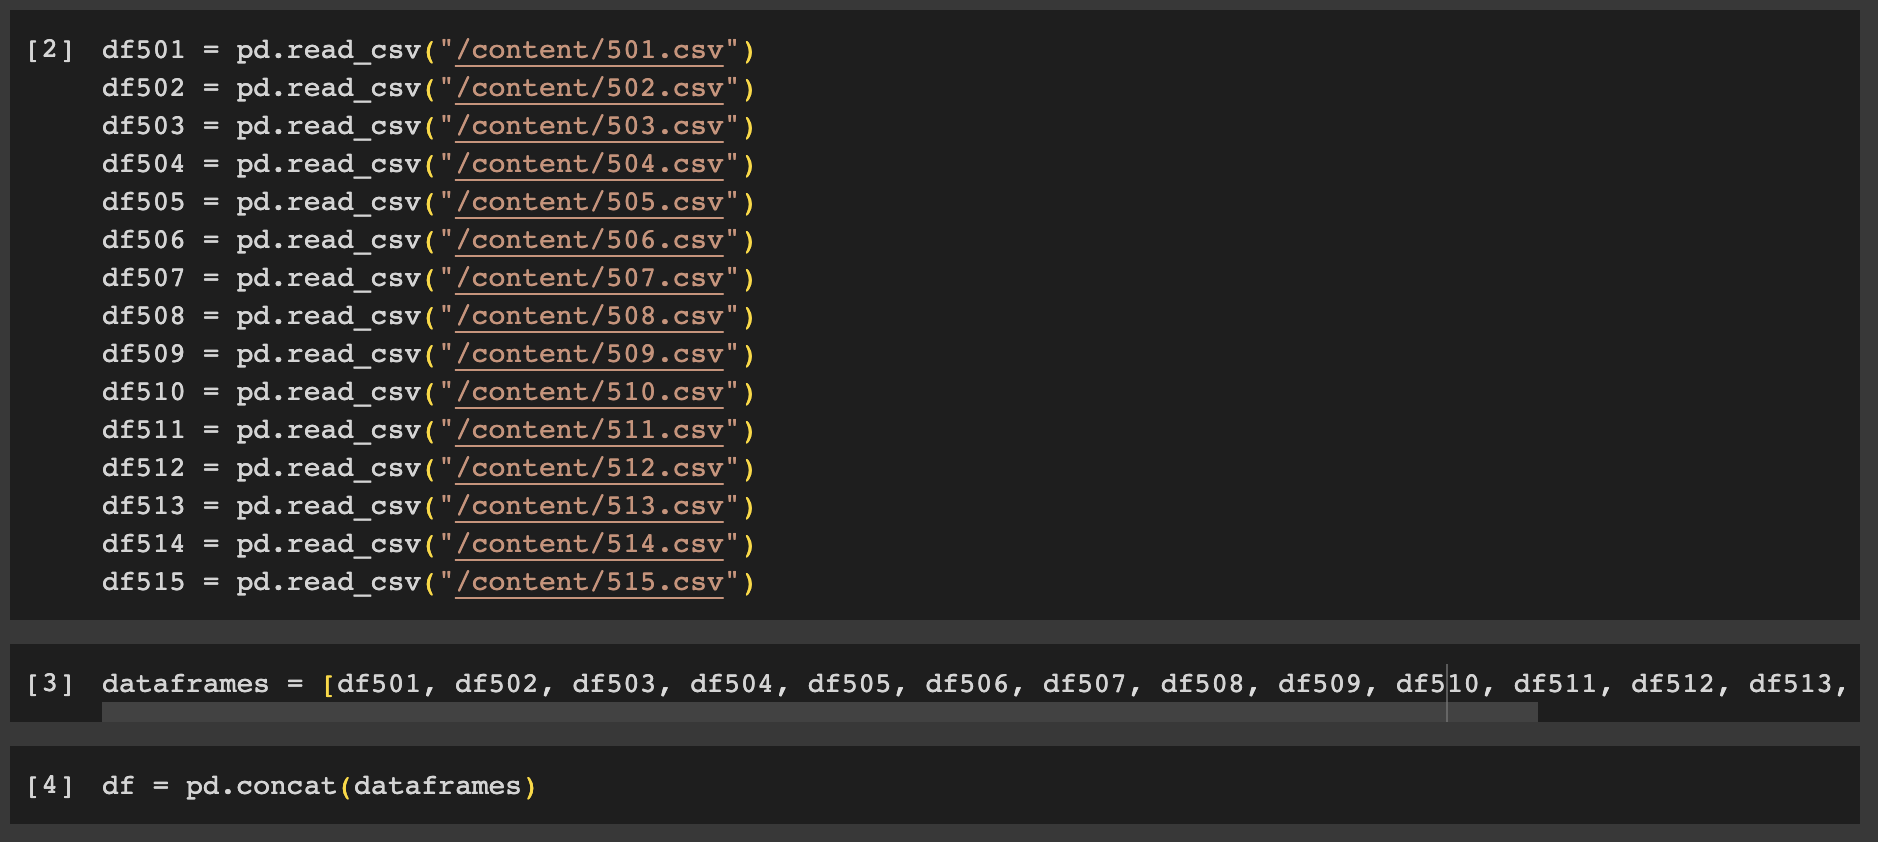
\includegraphics[scale=0.4]{/Users/manuelcardenas/Desktop/Latex/AI/images/intro1.png}
        \label{fig:intro1}
    \end{figure}




    \subsection{Exploratory Analysis}

    As you can see below we stated by simply undestanding the size of the sample, then print a summary of the data 
    in a table and understanding the type of data in three: object, float and integer. \pagebreak
    \begin{figure}[h]
        \centering
        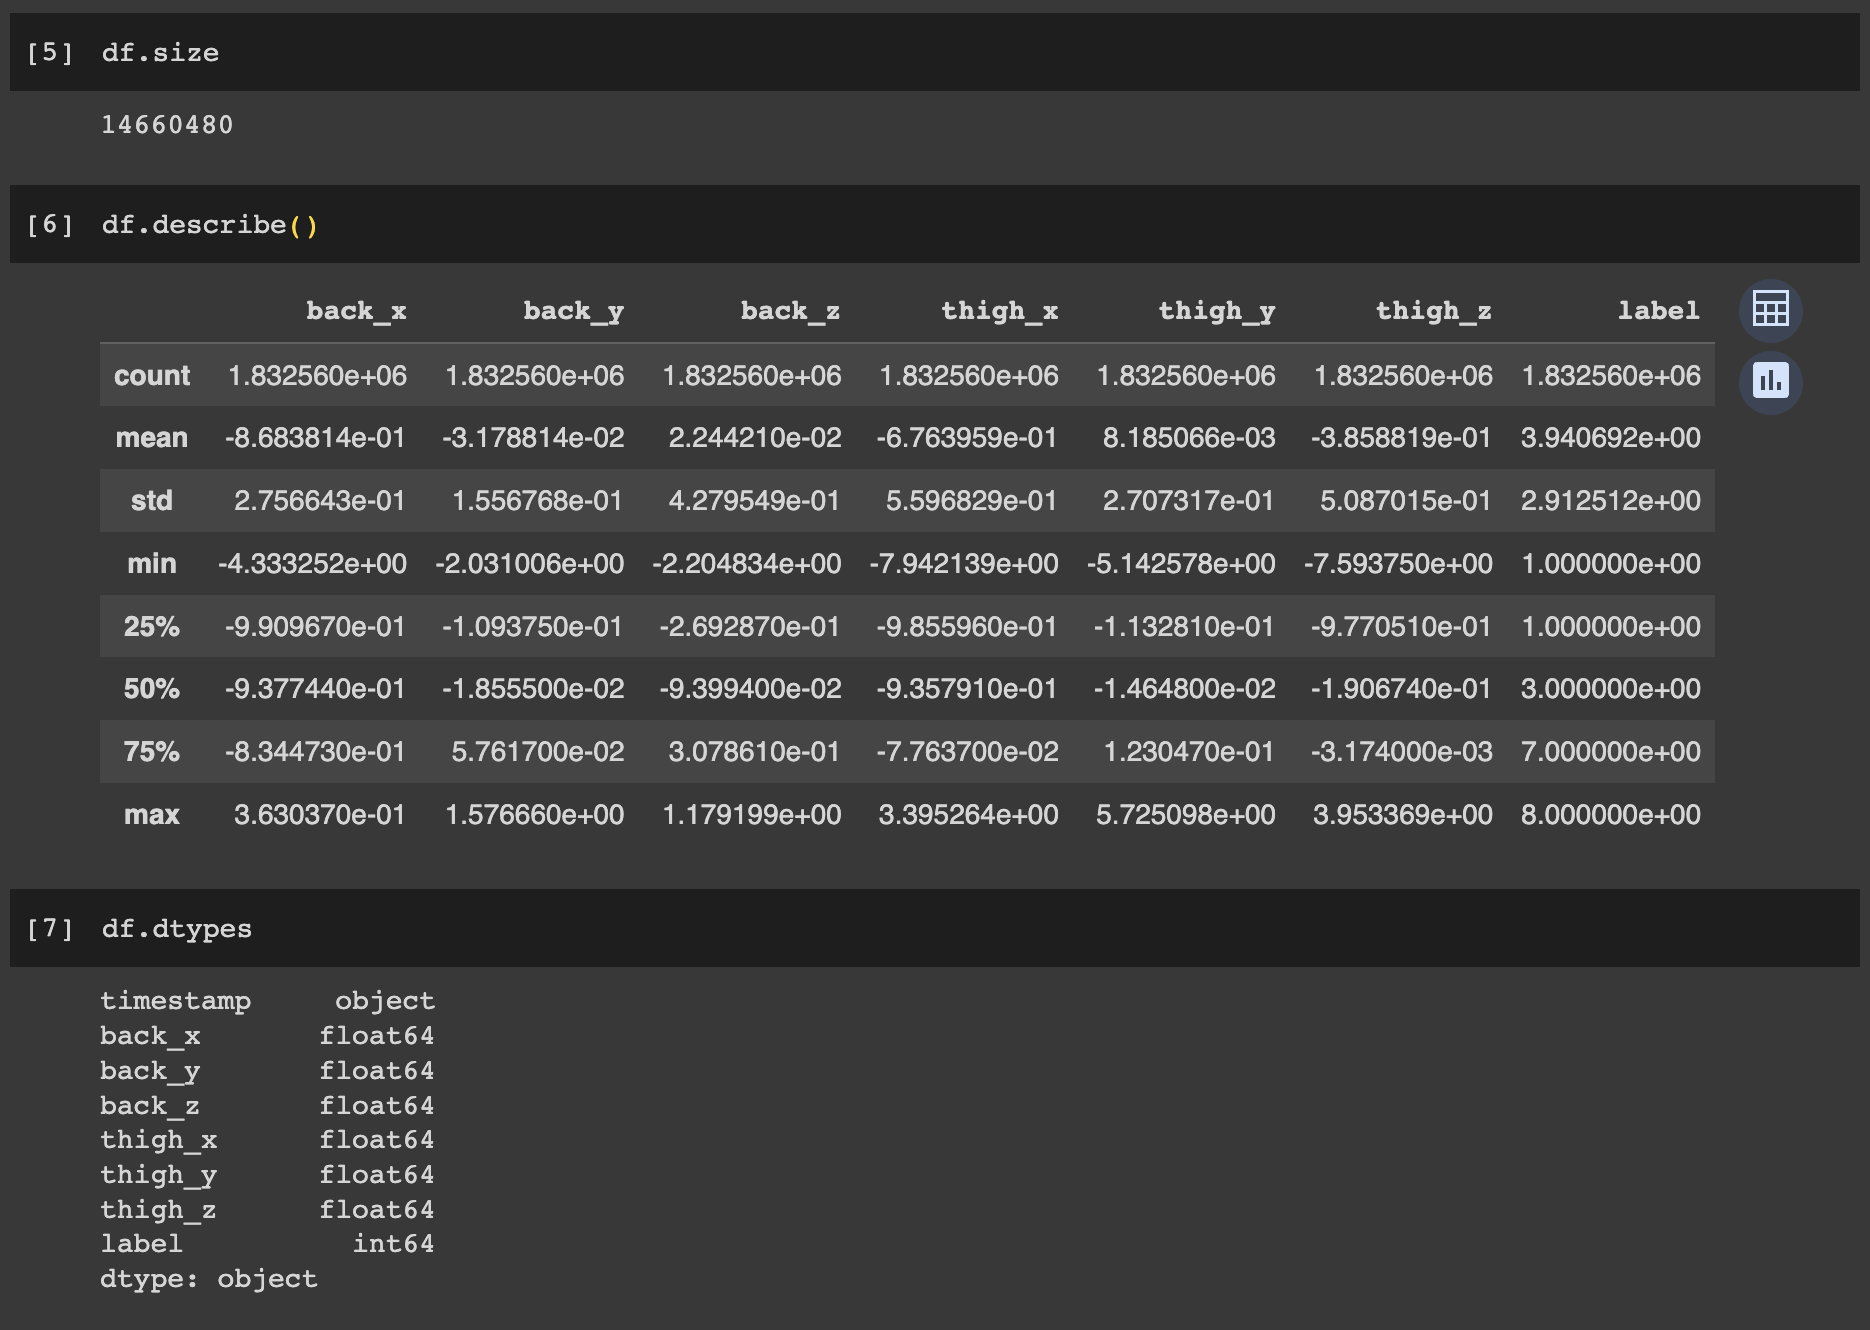
\includegraphics[scale=0.4]{/Users/manuelcardenas/Desktop/Latex/AI/images/intro2.png}
        \label{fig:intro2}
    \end{figure}




    As we can see there is no missng information in any of the columns, which in turn will save us a step for creating the model. 
    There we can also see that by uiing the function .unique() we are able to see the labels, which coincide with thoseis Kaggle. 
    It is divided as follows \\ \\
    1. walking \newline
    3. shuffling\newline
    4. ascending stairs\newline
    5. descending stairs \newline
    6. standing \newline
    7. sitting \newline
    8. lying \pagebreak
    \begin{figure}[h]
        \centering
        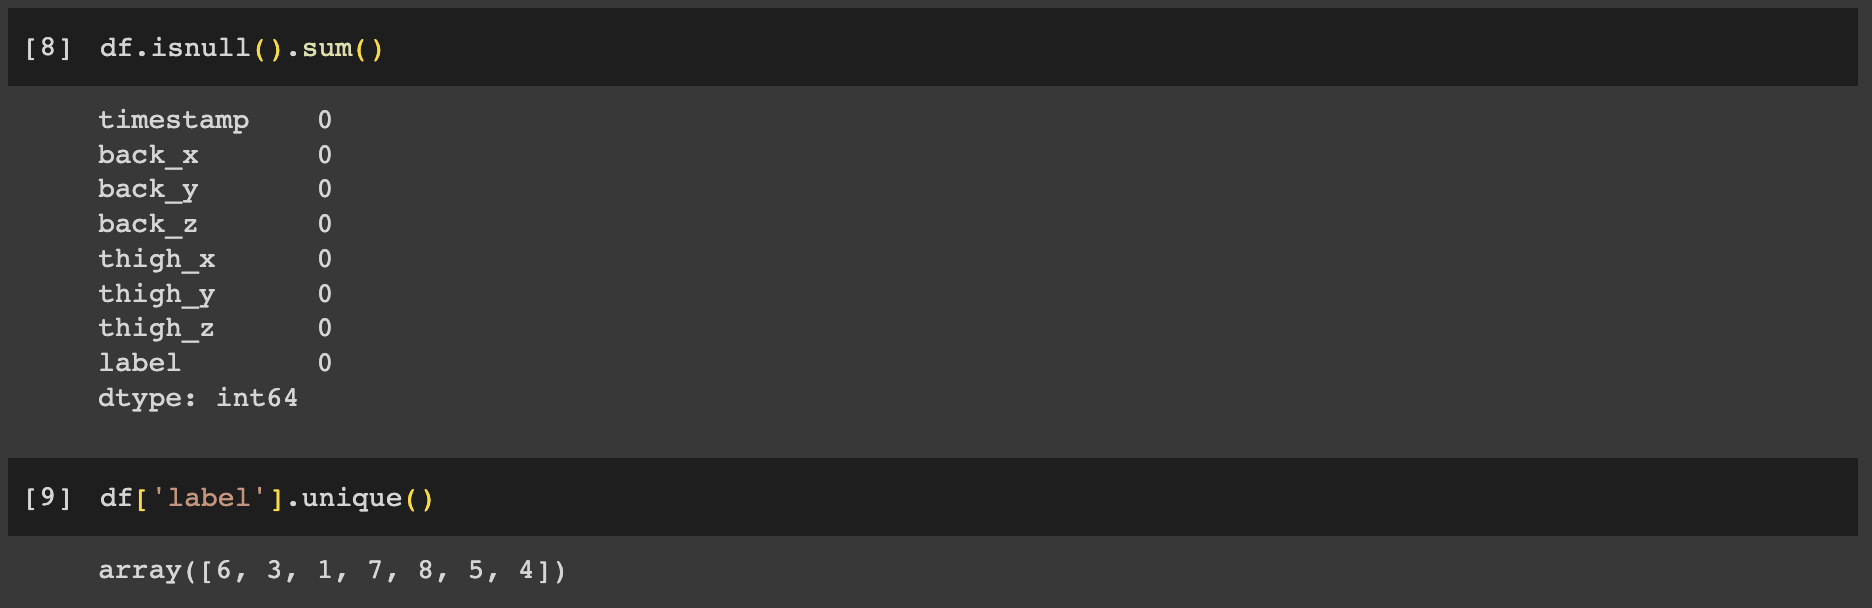
\includegraphics[scale=0.4]{/Users/manuelcardenas/Desktop/Latex/AI/images/intro3.png}
        \label{fig:intro3}
    \end{figure}






    It is also important to highlight that we manage to understand how the data is distributed within each label. 
    As we can see, the data is unfairly distributed among the lables. Therefore we must implement a balancing method in order 
    to advance with the perdiction method. Balancing data is crucial to prevent biased models, enhance generalization, ensure 
    fairness and equity and, most importantly improve the performance metrics of the method. By addressing data imbalances we are
    making the model more accurate and equitable predictions, essentialy making it more reliable and useful in real-world applications 
    while mitigating the negatve impact of class imbalances. \pagebreak
    \begin{figure}[h]
        \centering
        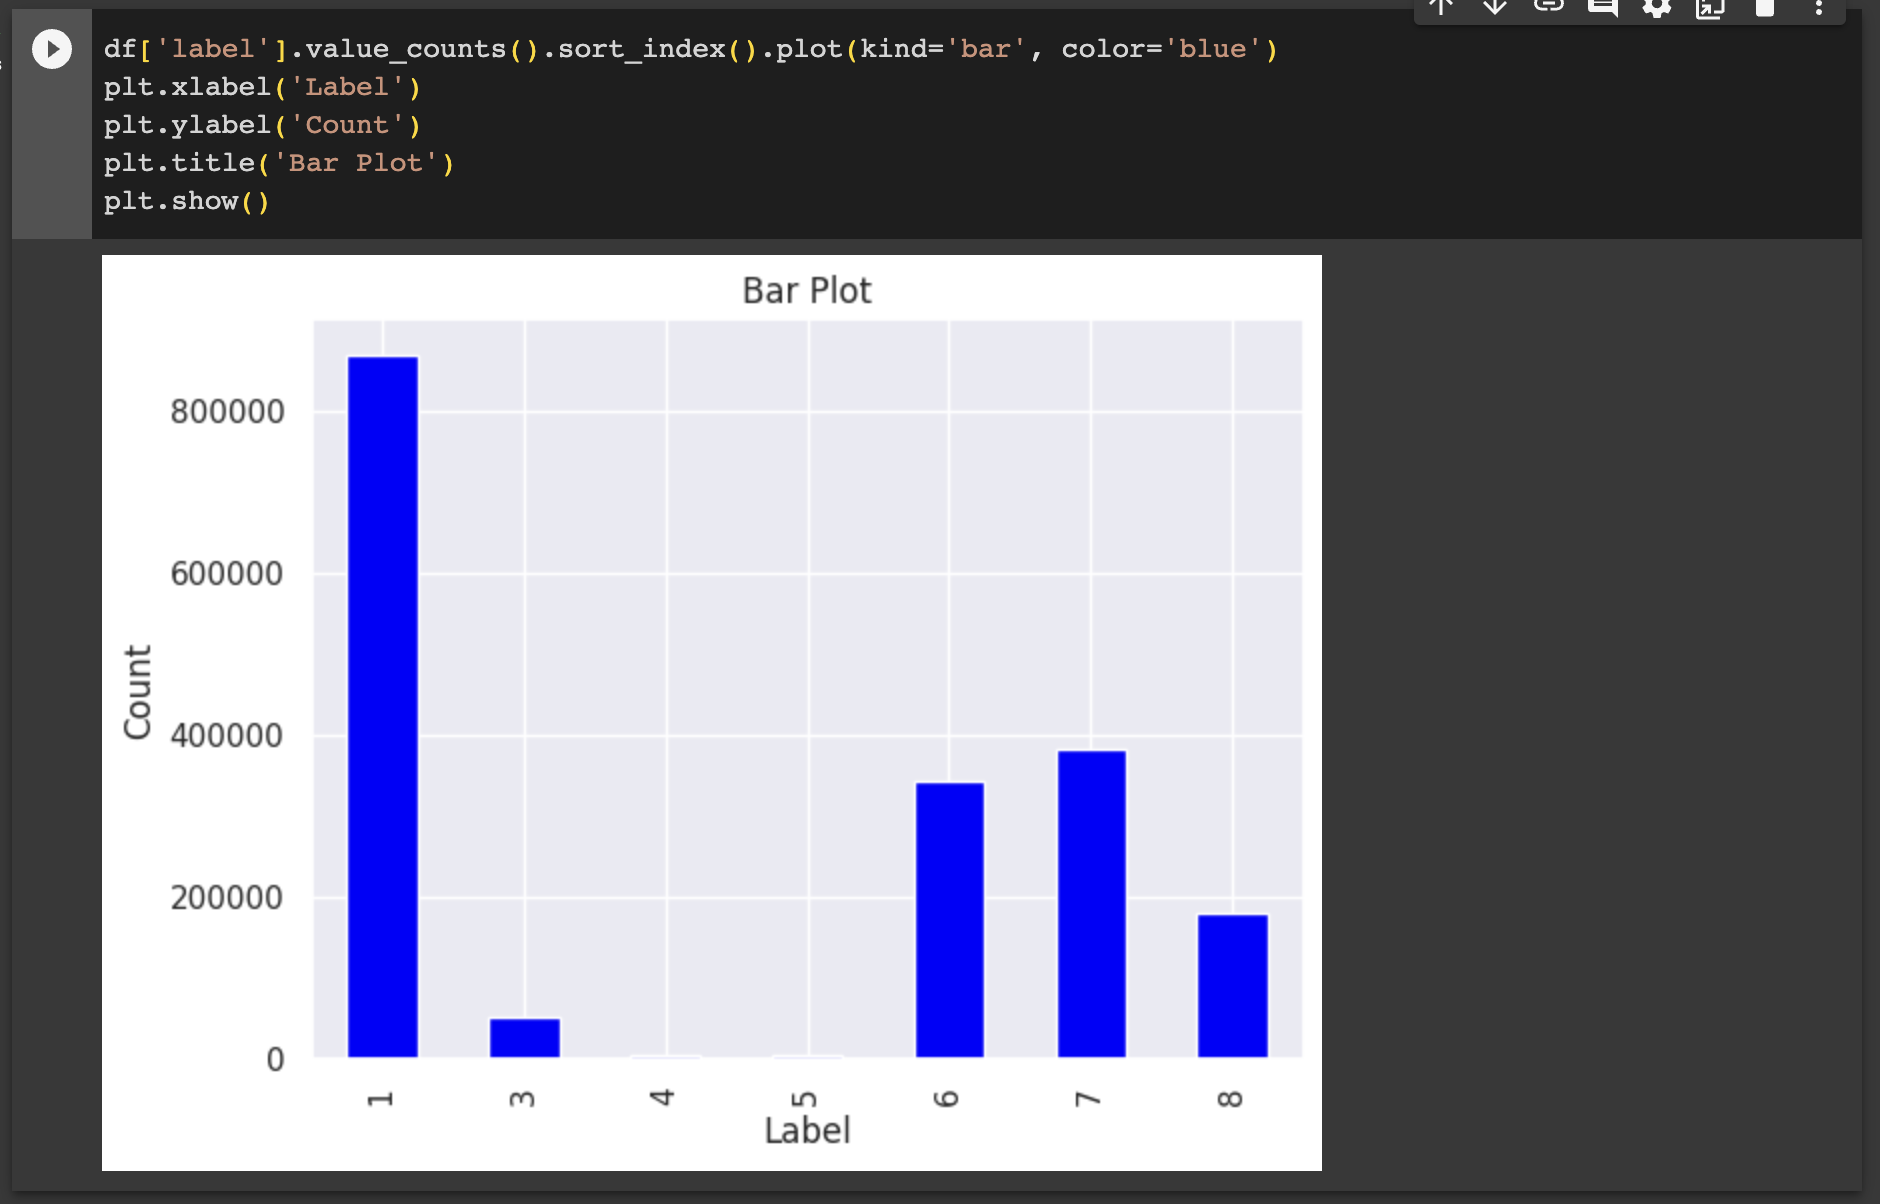
\includegraphics[scale=0.4]{/Users/manuelcardenas/Desktop/Latex/AI/images/intro4.png}
        \label{fig:intro4}
    \end{figure}





    Next we analized how the variables function in regard with the tieme. The code below graphs the data in labels 
    and shows how is acts as the time goes by. It is worth noting that this is merely a small sample of the Data Frame, 
    since running this code with the whole amount of data would take too long to display. However, we areable to see the 
    how each individual label acts in comparison to the rest. The amouont of time and movemente clearly displays the 
    relevance of some labels over others. Image:\pagebreak
    \begin{figure}[h]
        \centering
        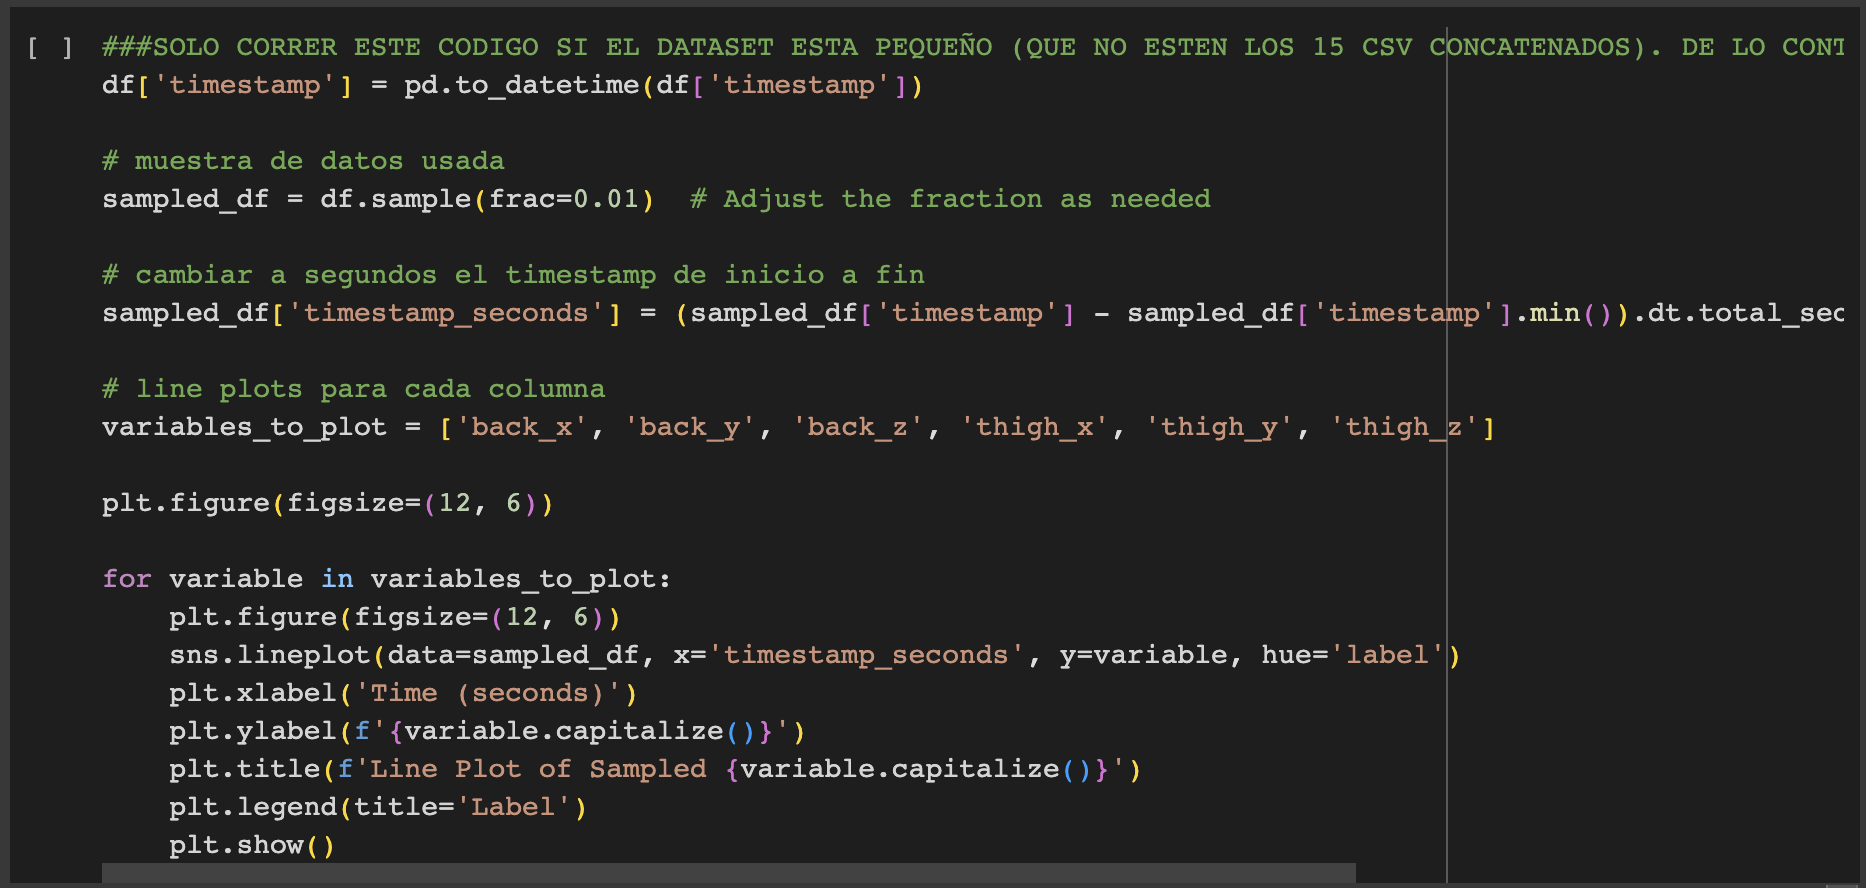
\includegraphics[scale=0.4]{/Users/manuelcardenas/Desktop/Latex/AI/images/intro5.png}
        \label{fig:intro5}
    \end{figure}

    Image:\pagebreak

    \begin{figure}[h]
        \centering
        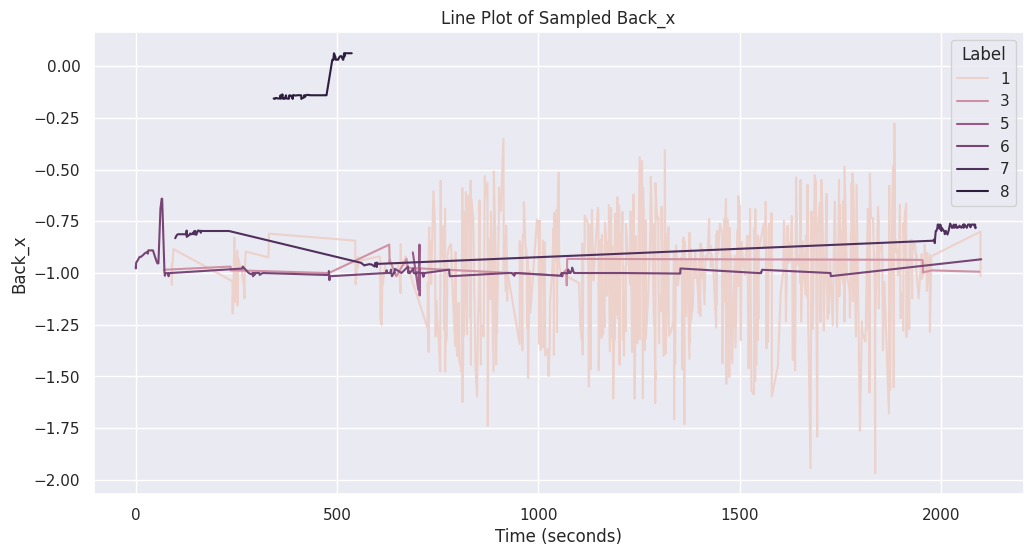
\includegraphics[scale=0.4]{/Users/manuelcardenas/Desktop/Latex/AI/images/intro6.png}
        \label{fig:intro6}
    \end{figure}

    

    \begin{figure}[h]
        \centering
        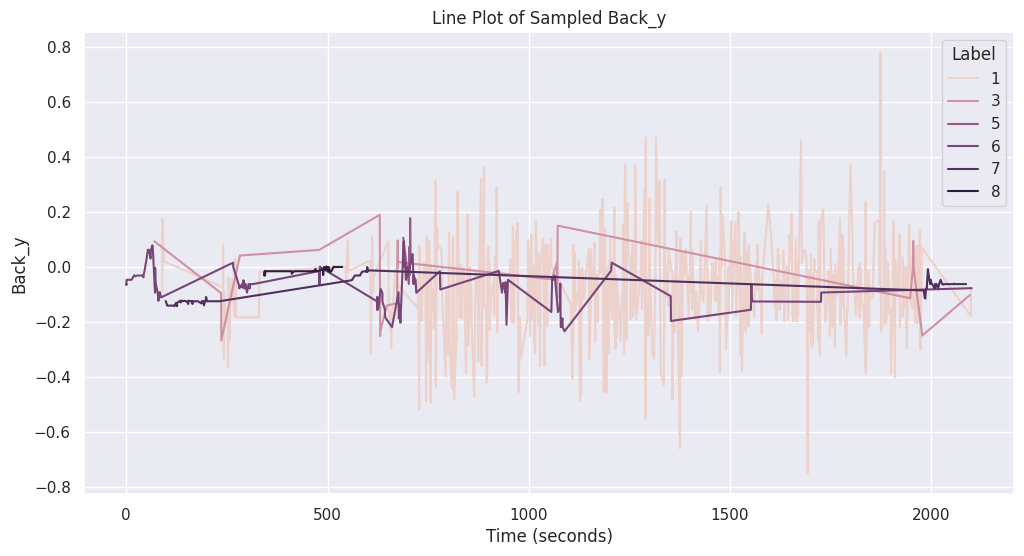
\includegraphics[scale=0.4]{/Users/manuelcardenas/Desktop/Latex/AI/images/intro7.png}
        \label{fig:intro7}
    \end{figure}

    Image:\pagebreak

    \begin{figure}[h]
        \centering
        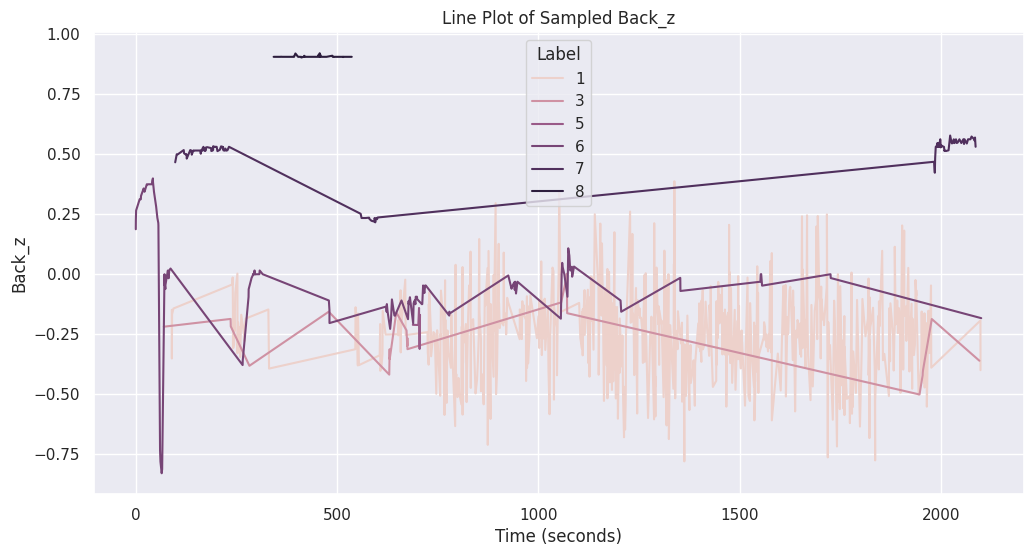
\includegraphics[scale=0.4]{/Users/manuelcardenas/Desktop/Latex/AI/images/intro8.png}
        \label{fig:intro8}
    \end{figure}

    

    \begin{figure}[h]
        \centering
        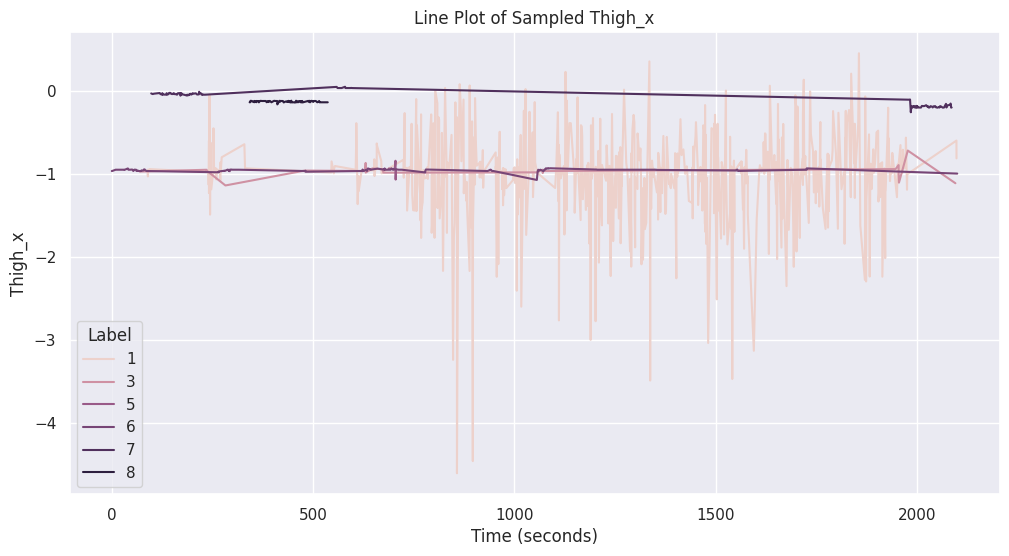
\includegraphics[scale=0.4]{/Users/manuelcardenas/Desktop/Latex/AI/images/intro9.png}
        \label{fig:intro9}
    \end{figure}

    Image:\pagebreak

    \begin{figure}[h]
        \centering
        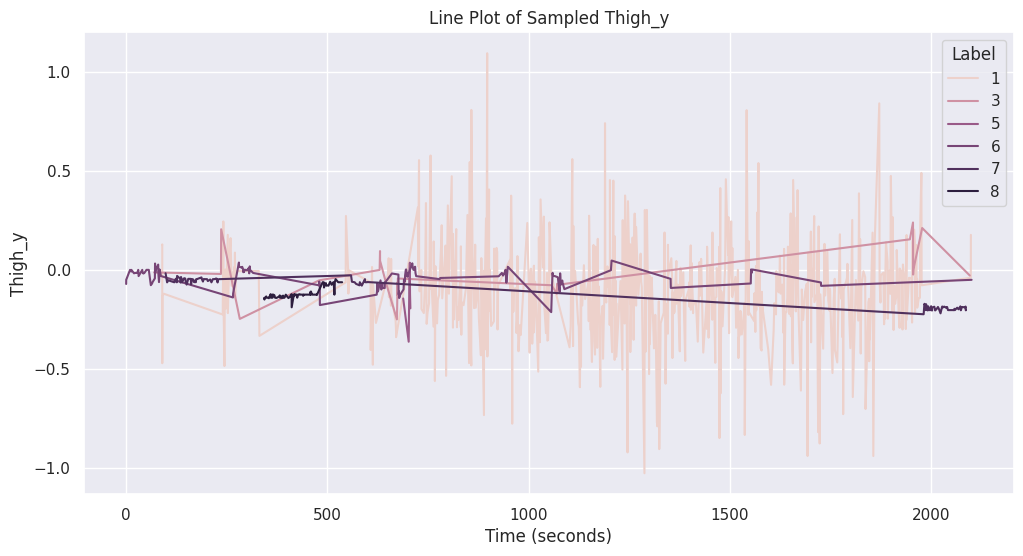
\includegraphics[scale=0.4]{/Users/manuelcardenas/Desktop/Latex/AI/images/intro10.png}
        \label{fig:intro10}
    \end{figure}


    Finally, we performed a Data Clusering in order to further understand how the data works.
    As we can see the data is very close together, mostly divided in three mayor labels, just as we saw prevosly, 
    however, it is worth noting the the data is closely tied together, there aren't any particular outliers that we need 
    to take into consideration.
    \begin{figure}[h]
        \centering
        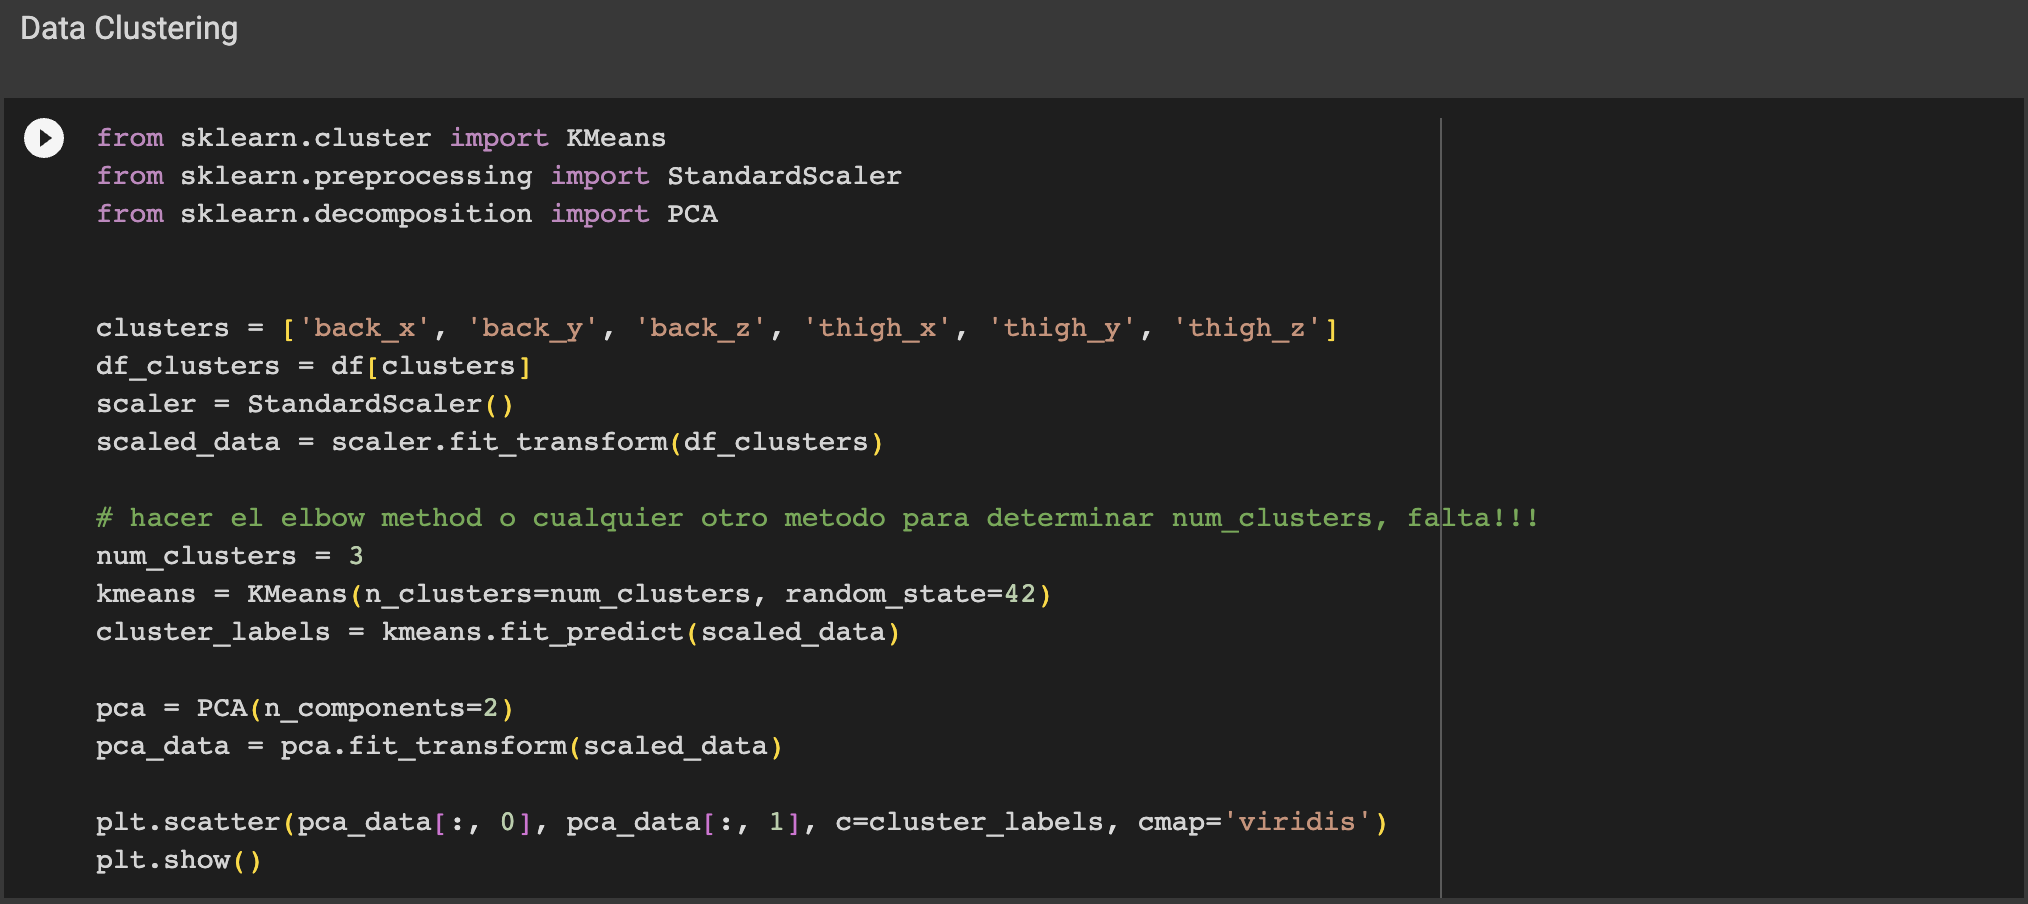
\includegraphics[scale=0.4]{/Users/manuelcardenas/Desktop/Latex/AI/images/intro11.png}
        \label{fig:intro11}
    \end{figure}

    Image:\pagebreak

    \begin{figure}[h]
        \centering
        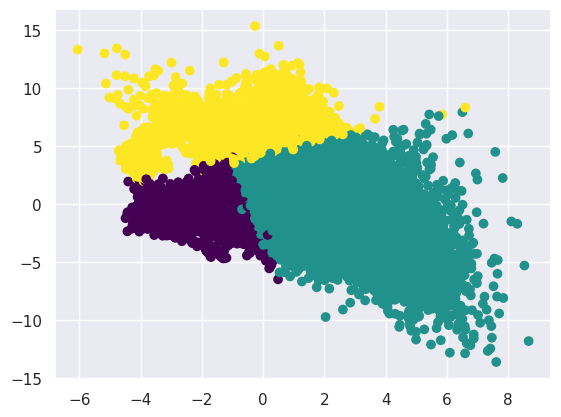
\includegraphics[scale=0.4]{/Users/manuelcardenas/Desktop/Latex/AI/images/intro12.png}
        \label{fig:intro12}
    \end{figure}

\section{Data Processing}
    \subsection{Unbalanced Analysis}

    First, we start by analyzing the model as it is,  with the data unbalanced. 
    The following code starts by setting up a stratified k-fold cross-validation, splitting the dataset into three folds 
    and shuffling the data. It employs a linear Support Vector Classifier (SVC) for training and prediction. During each fold, 
    it trains the model on a training subset and evaluates its performance on a validation subset, storing the true and 
    predicted labels. After the cross-validation, it concatenates the true and predicted labels from all folds and generates 
    a comprehensive classification report, presenting key classification metrics such as precision, recall, f1-score, and support 
    for each class. This report provides a consolidated view of the model's performance across all folds, offering insights into 
    its generalization capabilities and predictive accuracy on the given dataset. \pagebreak
    \begin{figure}[h]
        \centering
        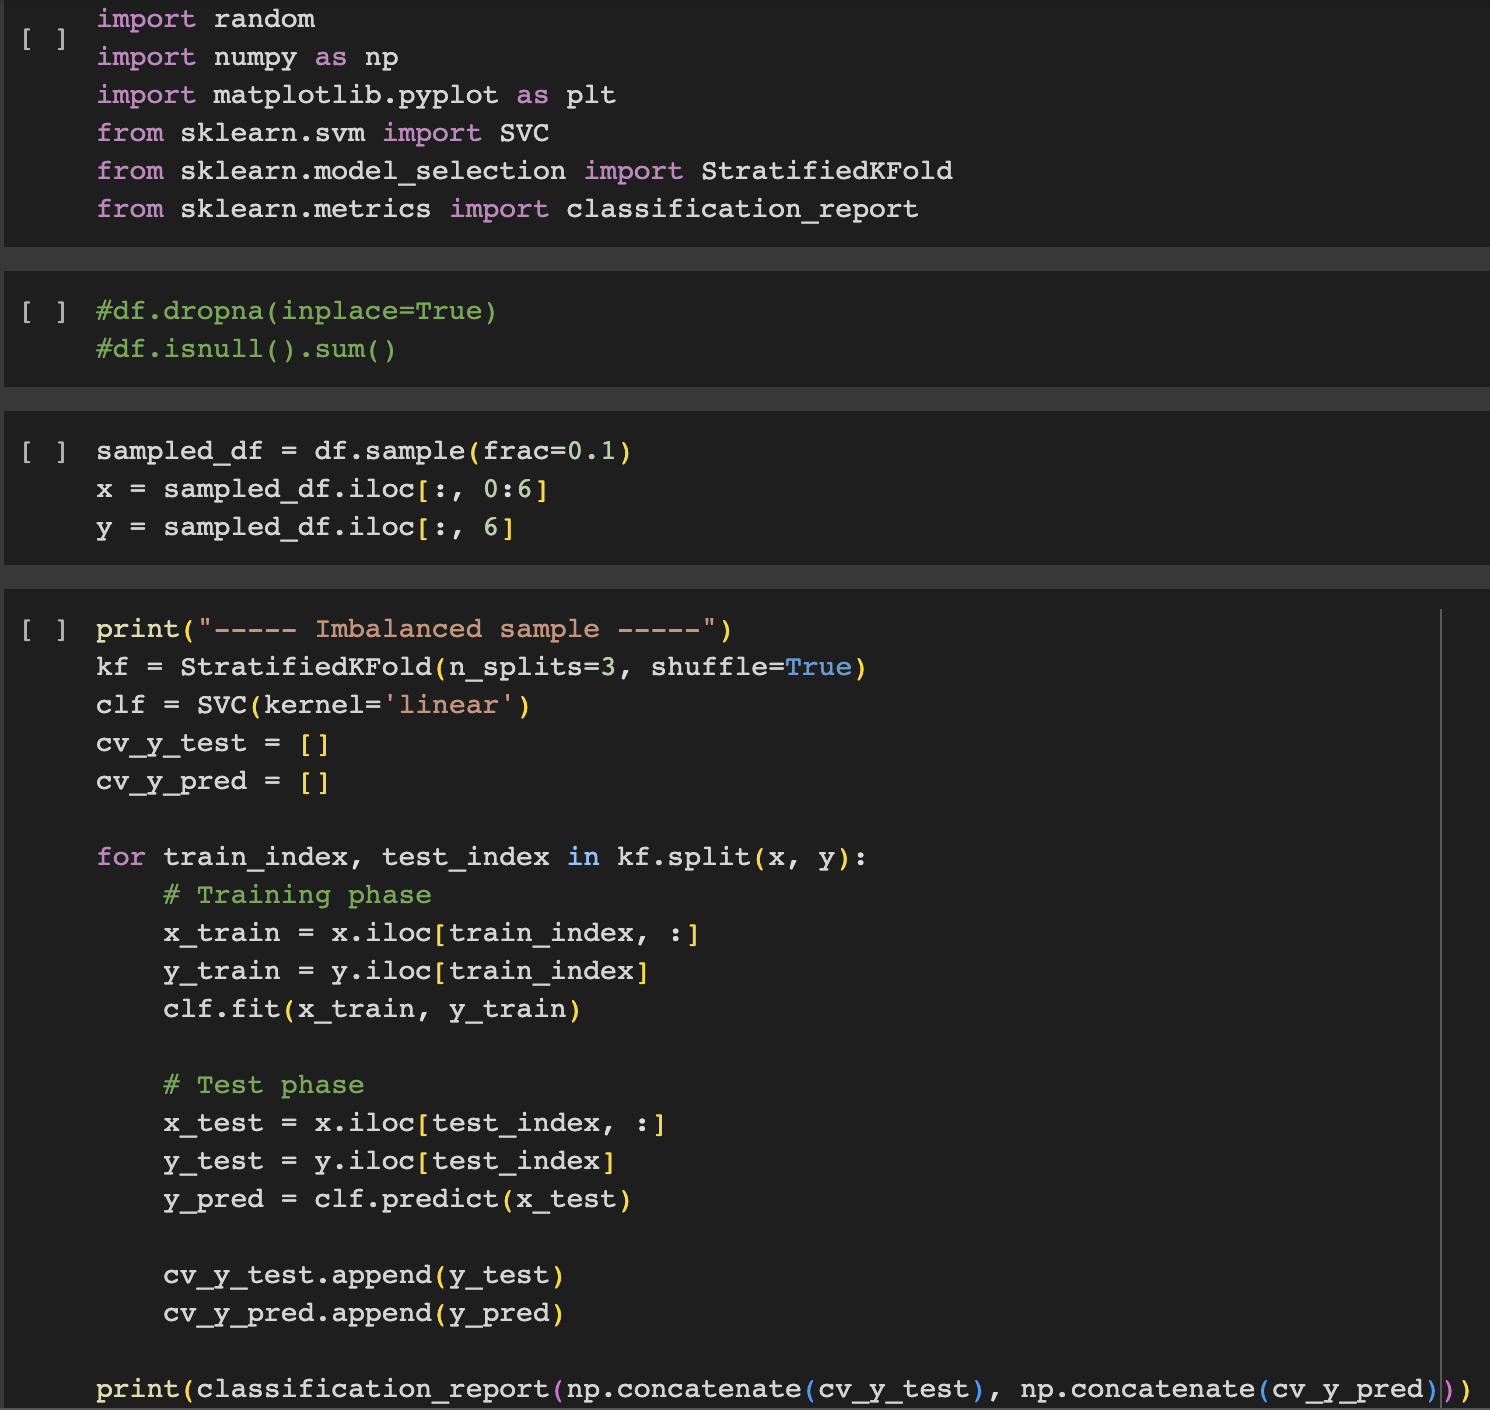
\includegraphics[scale=0.4]{/Users/manuelcardenas/Desktop/Latex/AI/images/ua1.png}
        \label{fig:ua1}
    \end{figure}
    
    As we can see by the results, the model as it is, with unbalanced data,  returns a poorly trained model. 
    The precision for two labels is approximately 98 percent, which is very good. However, the model is deficient in 
    predicting a precise answer for the remaining labels. Some even have 0 percent precision. This highlights the importance of creating 
    a balancing method in order to create an optimized and accurate model. \pagebreak
    \begin{figure}[h]
        \centering
        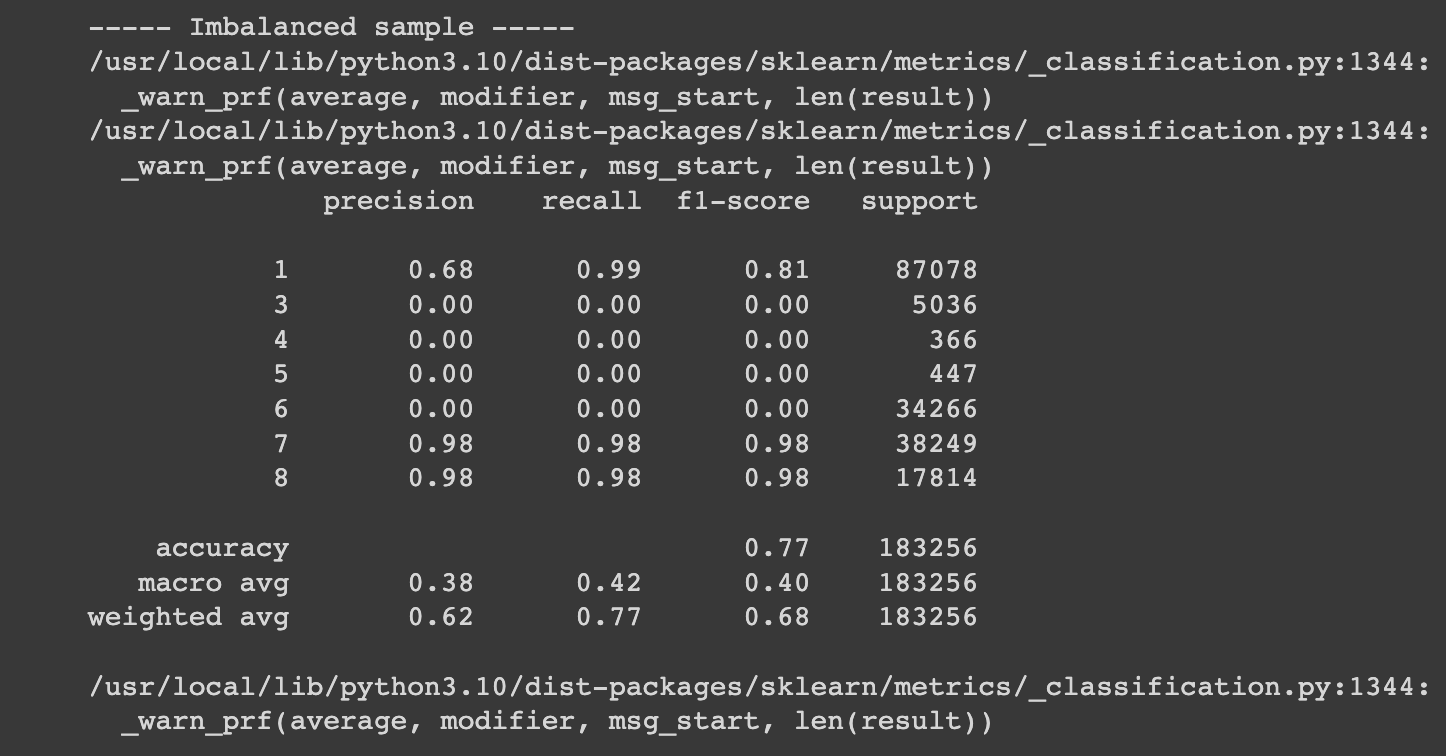
\includegraphics[scale=0.4]{/Users/manuelcardenas/Desktop/Latex/AI/images/ua2.png}
        \label{fig:ua2}
    \end{figure}


    \subsection{Balancing Methods}

    The following code begins by randomly sampling 10 percent of the rows from an original dataset and segregates 
    features and labels accordingly. It then focuses on addressing class imbalance in a classification task. The first approach, 
    "Upsampling," involves resampling the minority classes to equal the majority class in terms of sample count. The code accomplishes 
    this by duplicating samples from the minority class, achieving a more balanced dataset. The second strategy involves 
    utilizing a weighted loss function in conjunction with the Support Vector Classifier (SVC). By setting the class weights 
    to 'balanced,' the algorithm automatically adjusts these weights based on the class distribution in the training data, 
    effectively mitigating the imbalanced class issue. Both strategies aim to improve classification performance by enhancing 
    the model's ability to handle disparate class frequencies. The code concludes by presenting a detailed classification report, 
    offering insights into the model's performance across various evaluation metrics.\pagebreak
    \begin{figure}[h]
        \centering
        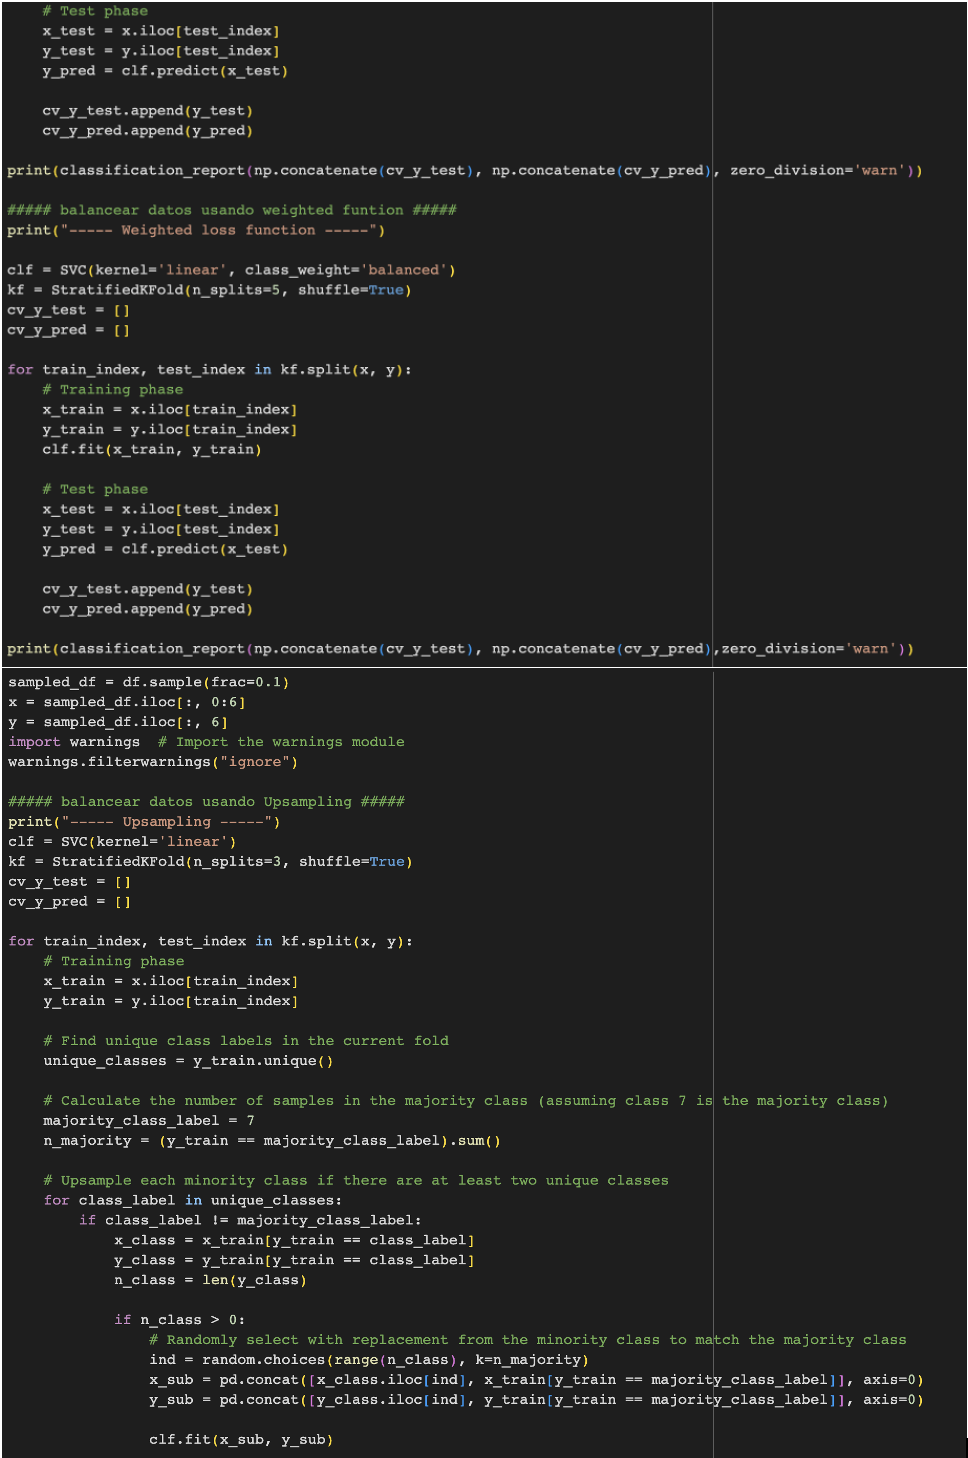
\includegraphics[scale=0.5]{/Users/manuelcardenas/Desktop/Latex/AI/images/bm1.png}
        \label{fig:bm1}
    \end{figure}

    The result displays that although the methods did show some progress and optimized the unbalane defficiency, 
    it's still not the best solution for dealing the problem. The precision stil wrong, having some labels with 0 precision. \pagebreak
    \begin{figure}[h]
        \centering
        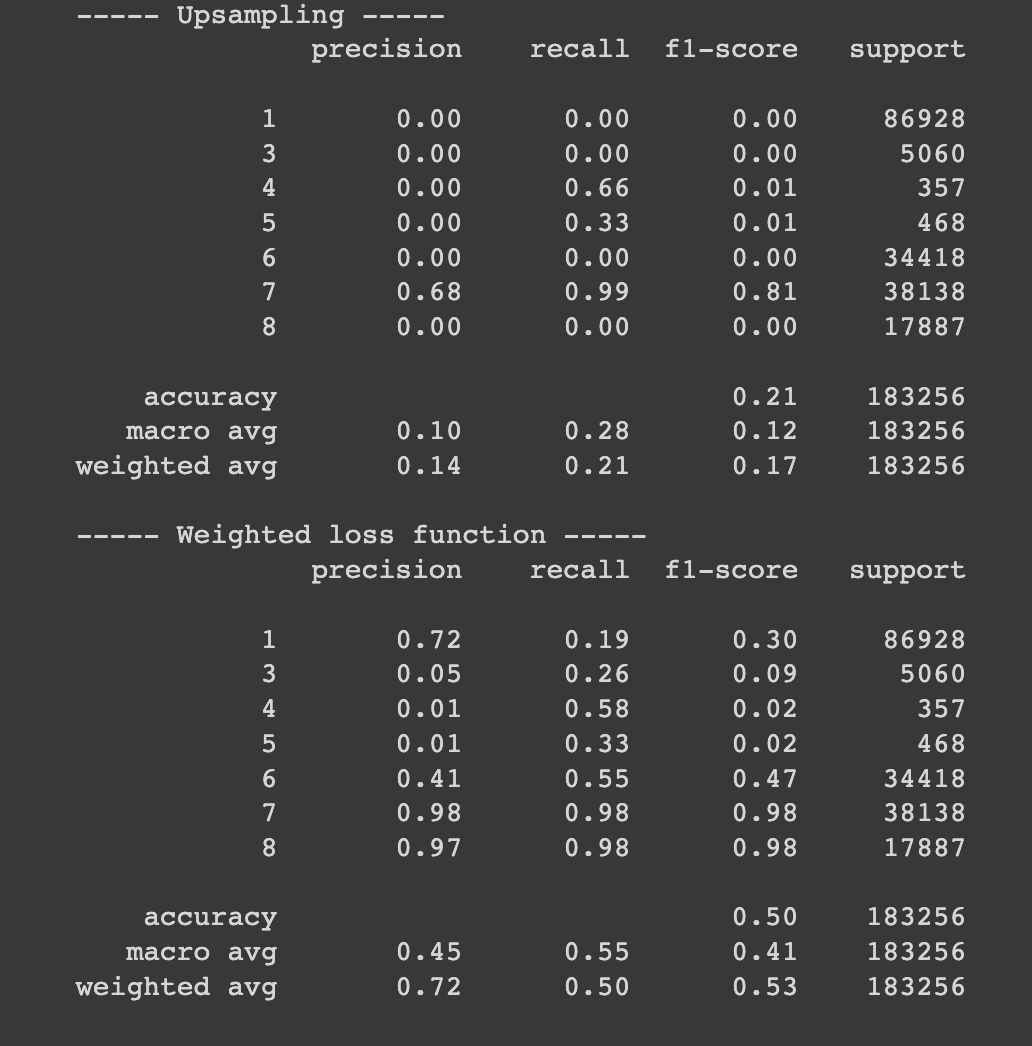
\includegraphics[scale=0.4]{/Users/manuelcardenas/Desktop/Latex/AI/images/bm2.png}
        \label{fig:bm2}
    \end{figure}

    \subsection{Methods}

    The next code conducts a comprehensive evaluation of multiple machine learning classifiers 
    (linear SVM, RBF SVM, KNN, Decision Tree, Linear Discriminant Analysis, Random Forest, Gradient Boosting, and Polynomial SVM) 
    on the dataset. The dataset is initially sampled, and features and labels are extracted. Each classifier is trained and evaluated 
    using 3-fold cross-validation. The evaluation involves training on a subset of the data and testing on another, followed by 
    generating a classification report detailing precision, recall, F1-score, and support metrics for each class. The main goal is 
    to assess and compare the performance of these classifiers on the dataset.\pagebreak

    Linear SVM
    \begin{figure}[h]
        \centering
        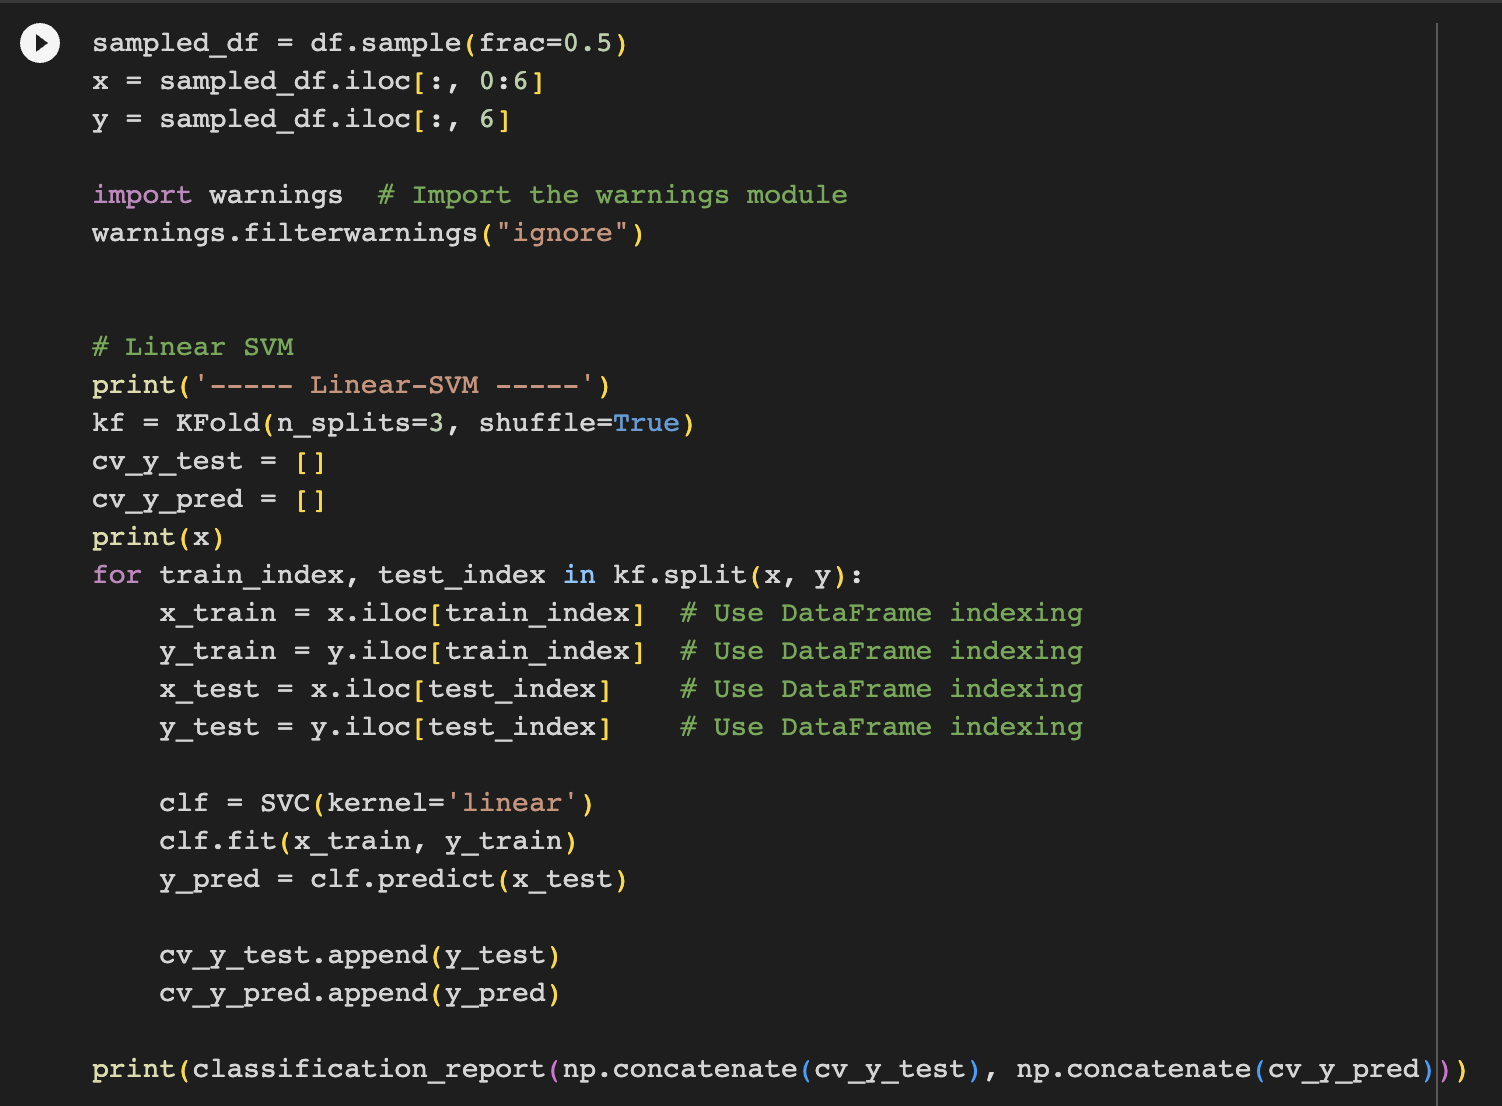
\includegraphics[scale=0.4]{/Users/manuelcardenas/Desktop/Latex/AI/images/m1.png}
        \label{fig:m1}
    \end{figure}

    RBF SVM \pagebreak
    \begin{figure}[h]
        \centering
        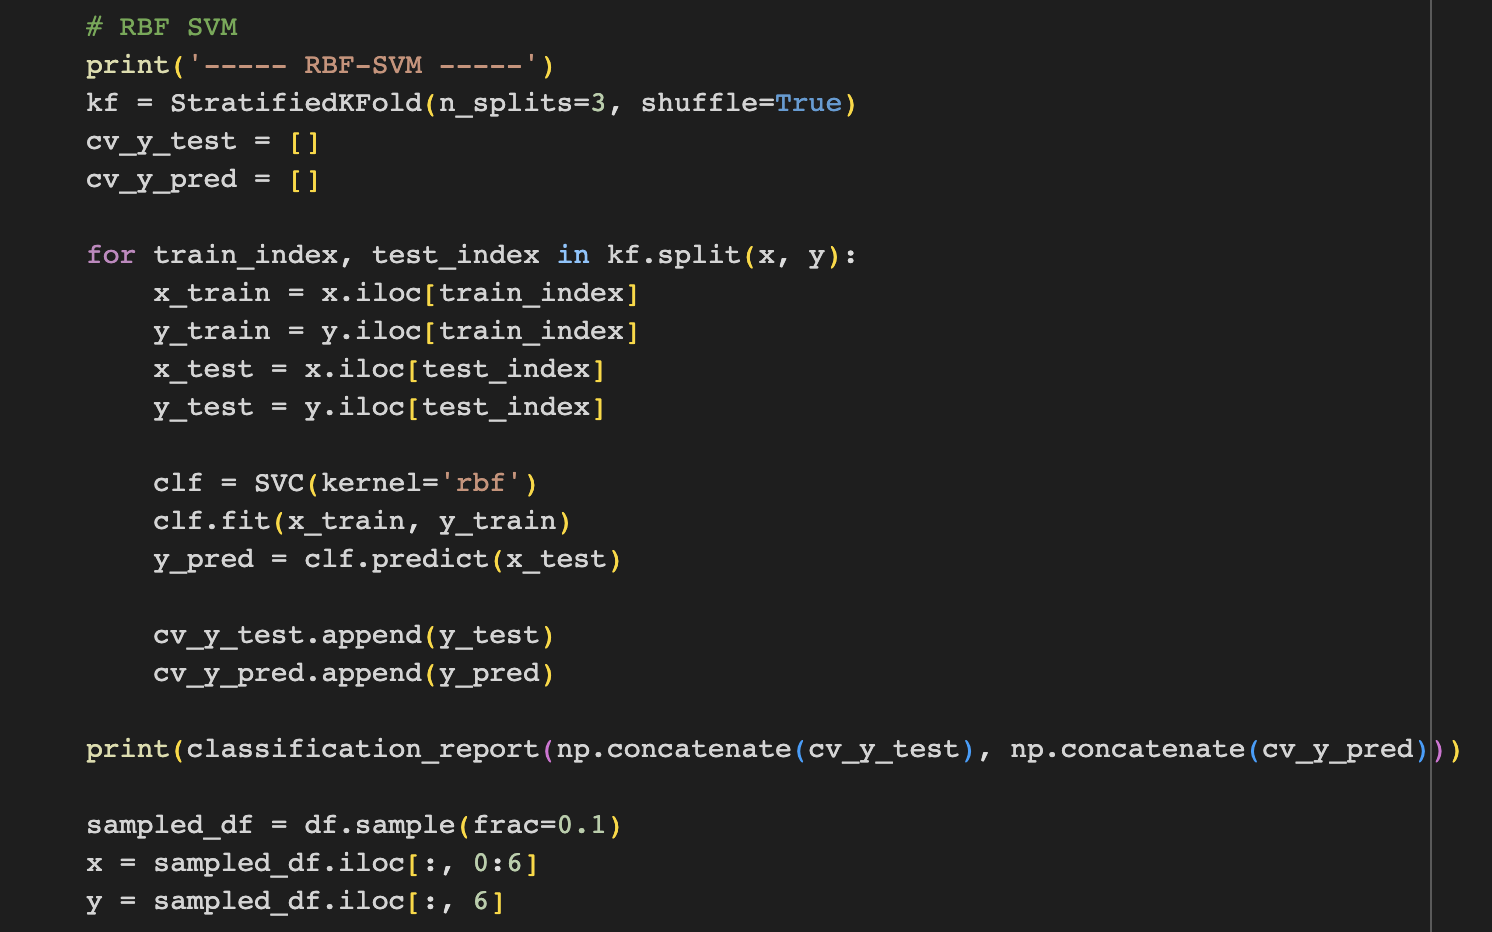
\includegraphics[scale=0.4]{/Users/manuelcardenas/Desktop/Latex/AI/images/m2.png}
        \label{fig:m2}
    \end{figure}

    KNN
    \begin{figure}[h]
        \centering
        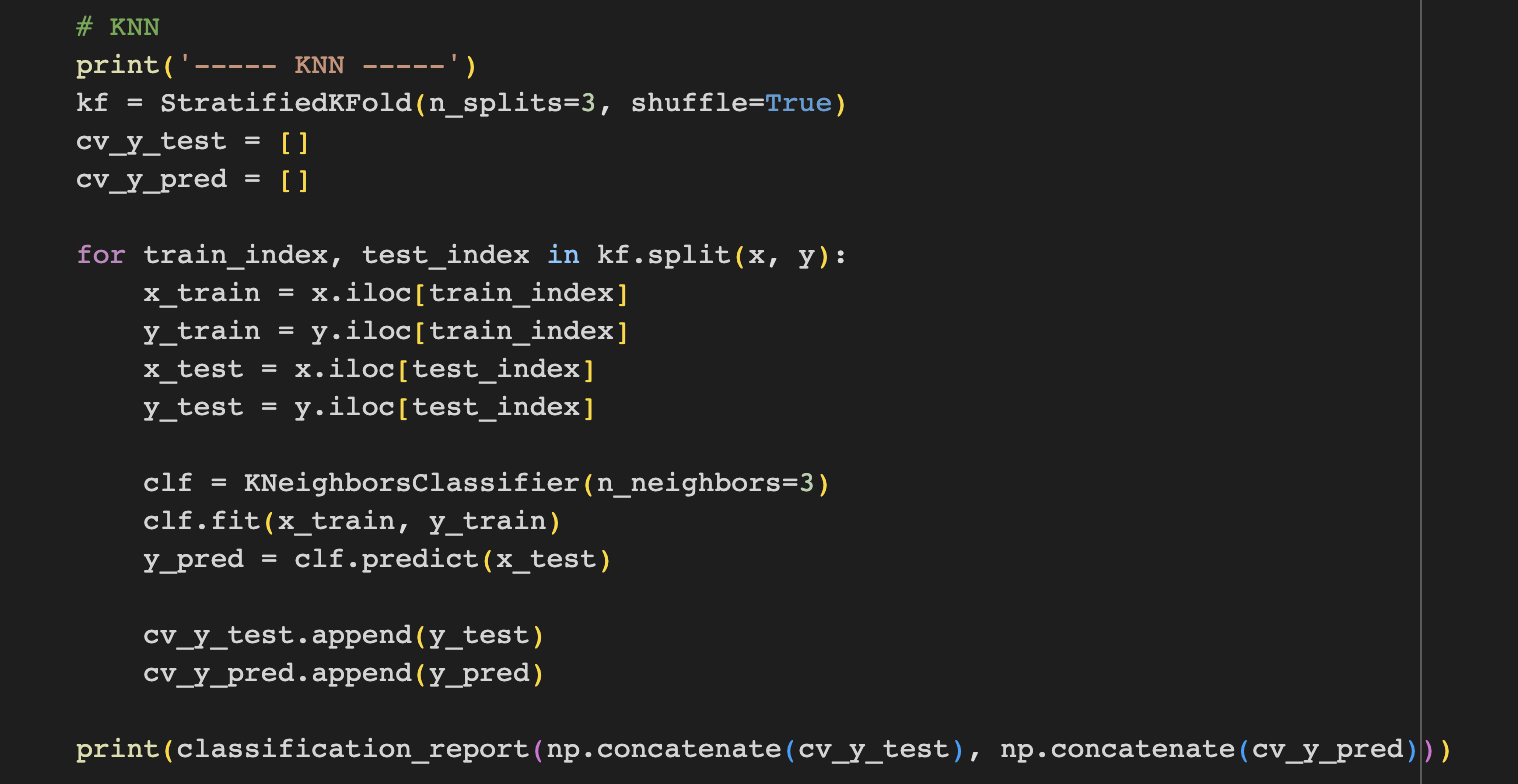
\includegraphics[scale=0.4]{/Users/manuelcardenas/Desktop/Latex/AI/images/m3.png}
        \label{fig:m3}
    \end{figure}

    Decision Tree\pagebreak
    \begin{figure}[h]
        \centering
        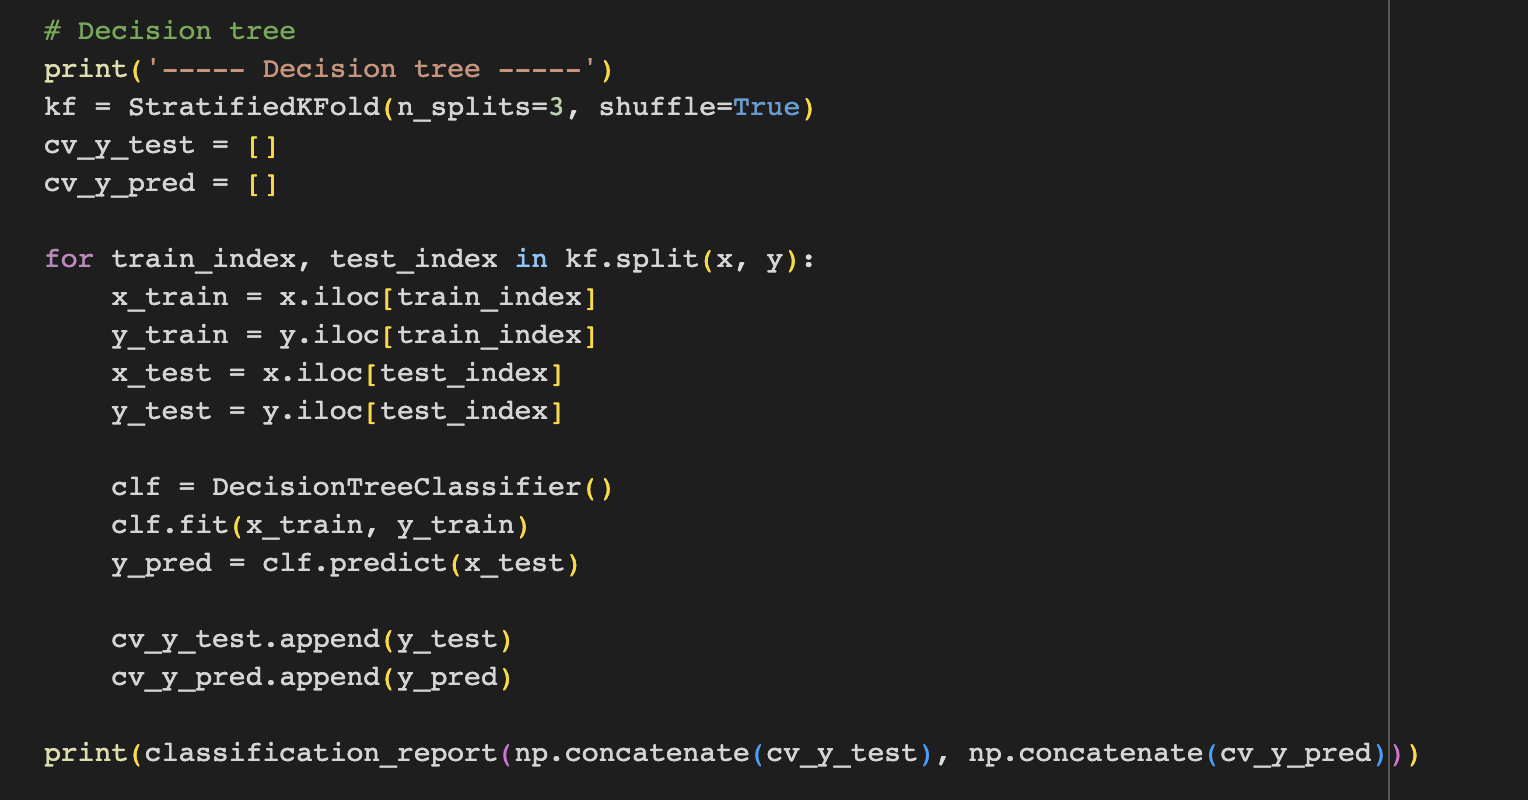
\includegraphics[scale=0.4]{/Users/manuelcardenas/Desktop/Latex/AI/images/m4.png}
        \label{fig:m4}
    \end{figure}

    Linear Discriminant Analysis
    \begin{figure}[h]
        \centering
        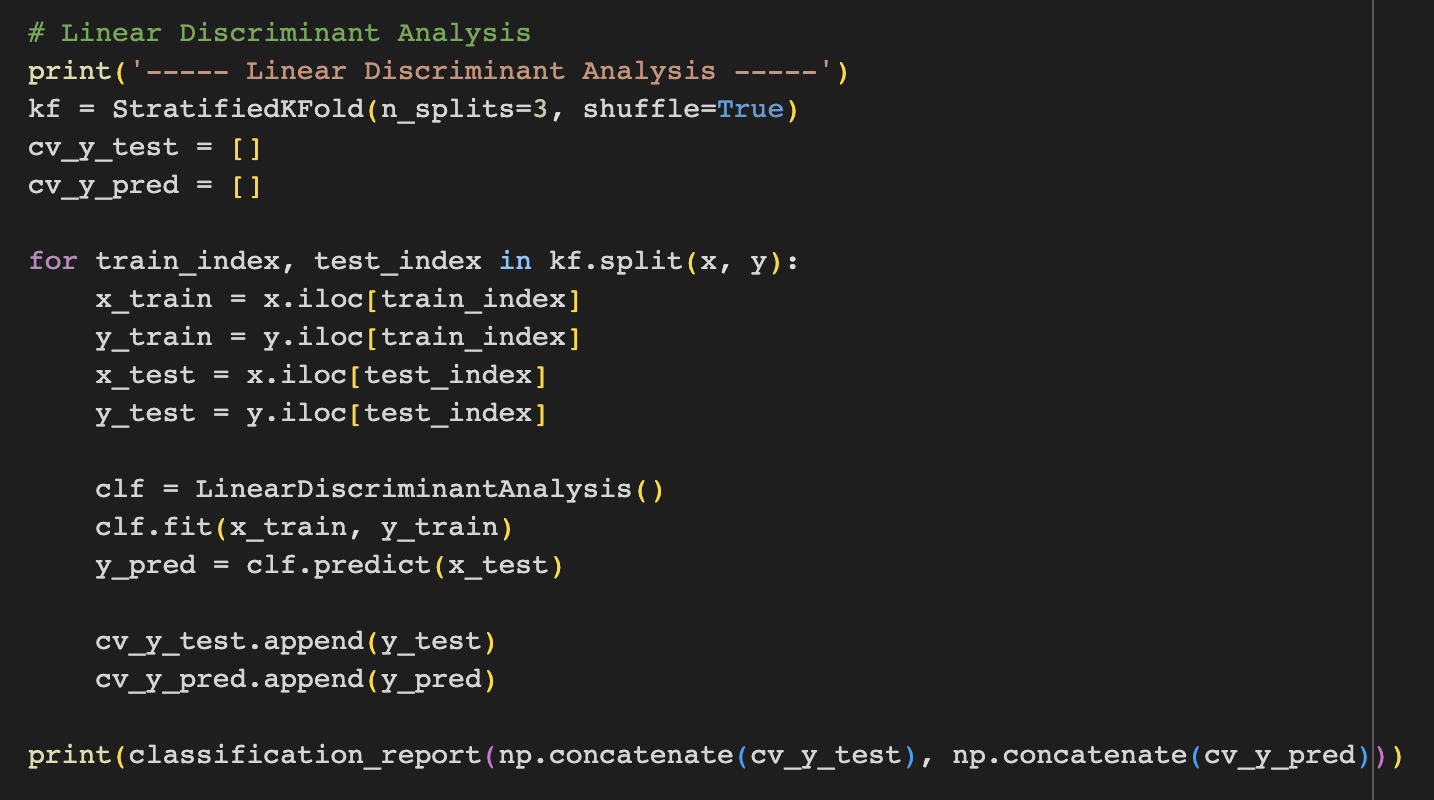
\includegraphics[scale=0.4]{/Users/manuelcardenas/Desktop/Latex/AI/images/m5.png}
        \label{fig:m5}
    \end{figure}

    Random Forest\pagebreak
    \begin{figure}[h]
        \centering
        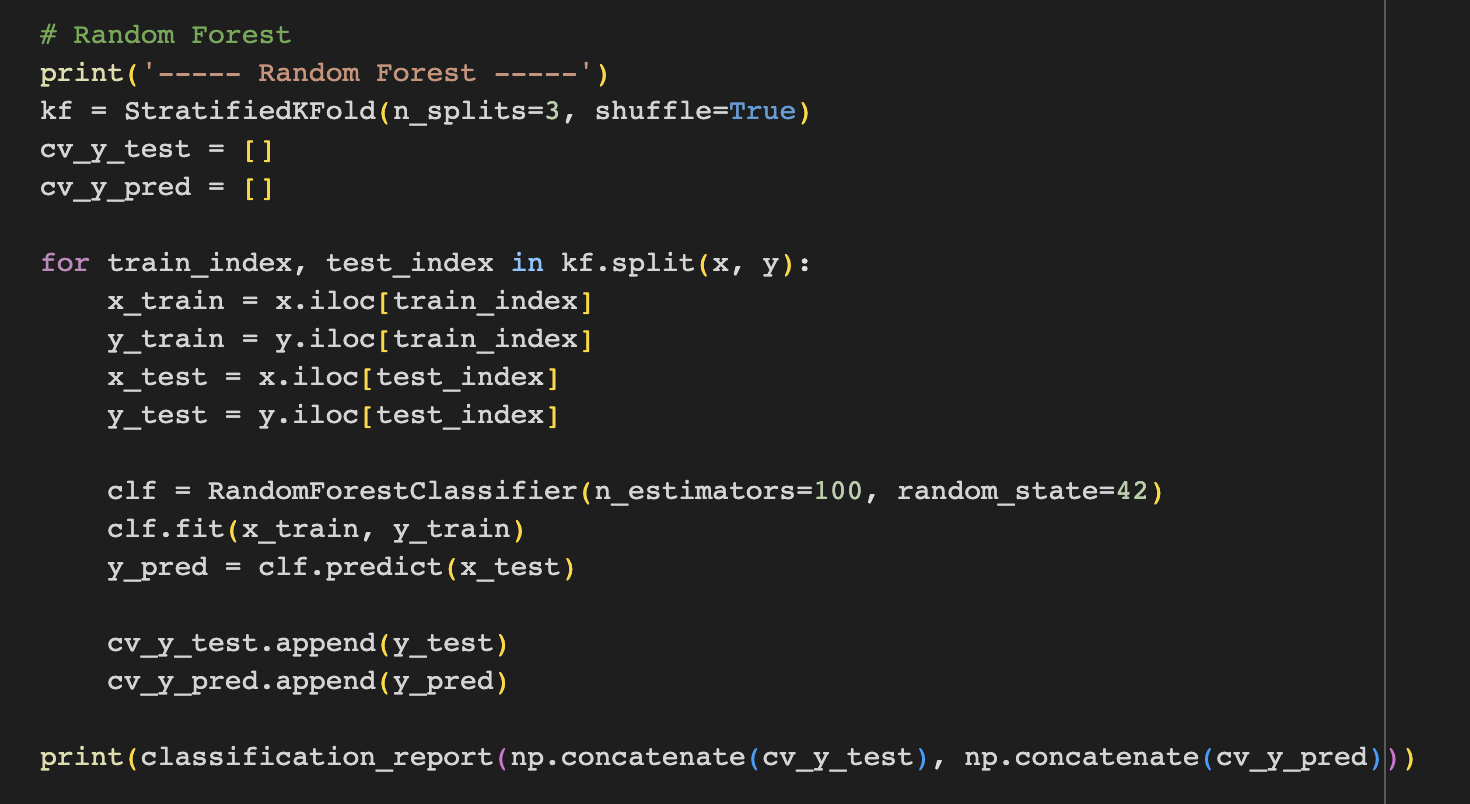
\includegraphics[scale=0.4]{/Users/manuelcardenas/Desktop/Latex/AI/images/m6.png}
        \label{fig:m6}
    \end{figure}

    Gradient Boosting
    \begin{figure}[h]
        \centering
        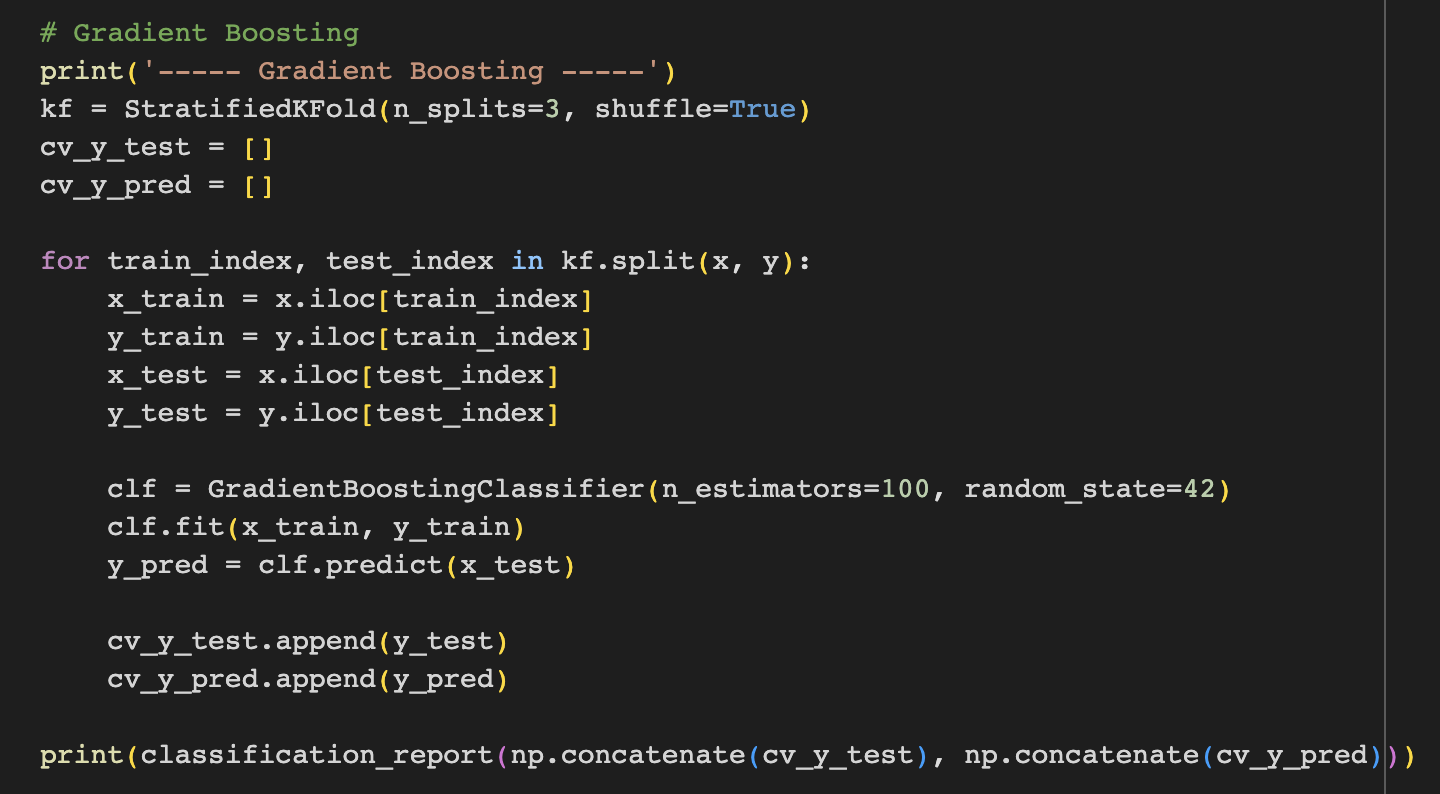
\includegraphics[scale=0.4]{/Users/manuelcardenas/Desktop/Latex/AI/images/m7.png}
        \label{fig:m7}
    \end{figure}

    SVM with Kernel Polynomial\pagebreak
    \begin{figure}[h]
        \centering
        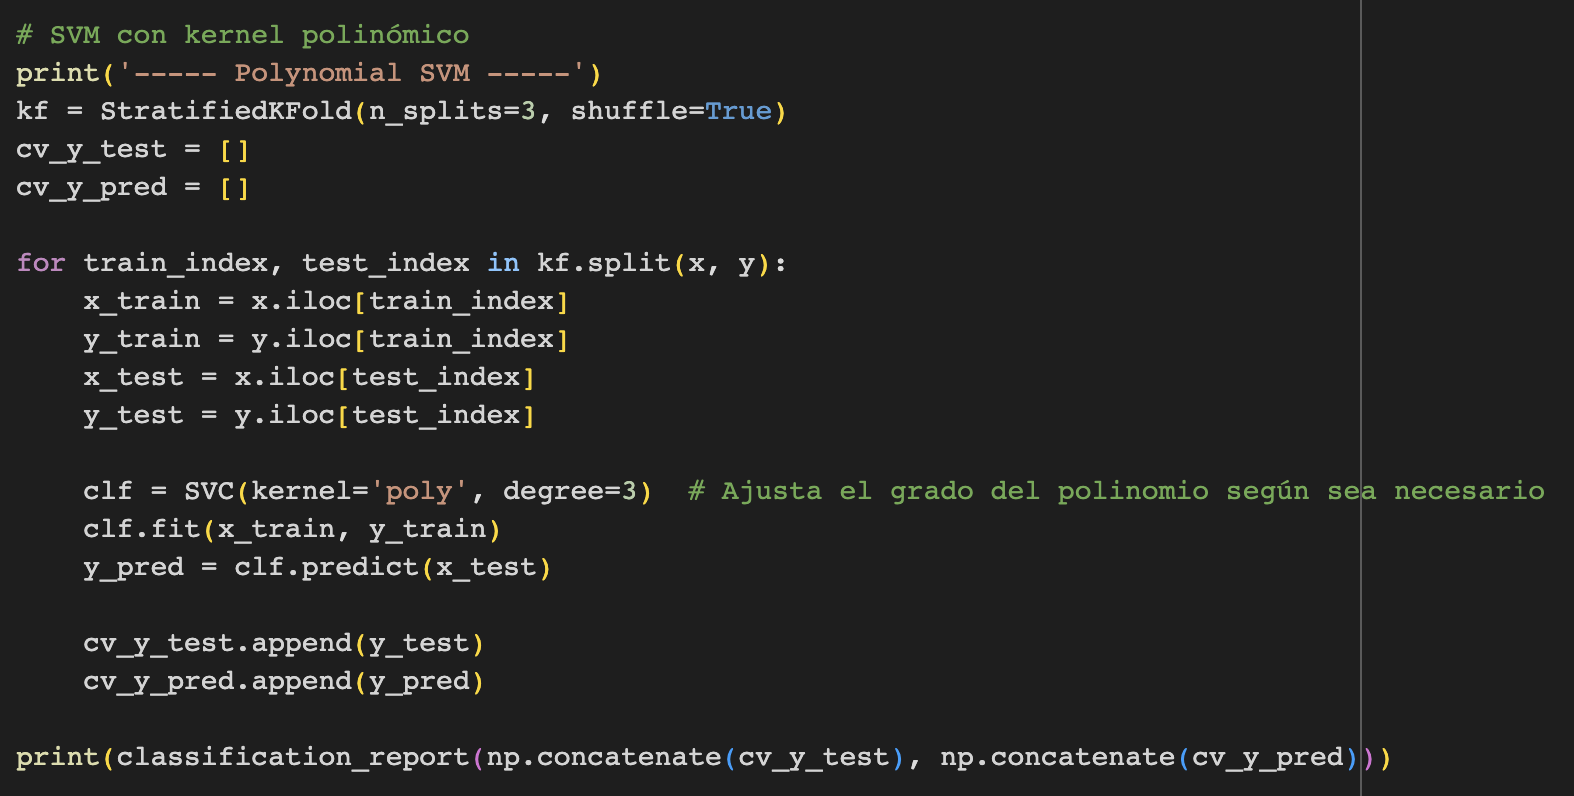
\includegraphics[scale=0.4]{/Users/manuelcardenas/Desktop/Latex/AI/images/m8.png}
        \label{fig:m8}
    \end{figure}

    The result display that the best model is the Random Forest. It shows the best precision overall in all the labels.
     The worst being of 0.53 and the best of 1.00. However, the recall is still pretty deficient on labels: 3, 4, and 5. \pagebreak
     Linear SVM
    \begin{figure}[h]
        \centering
        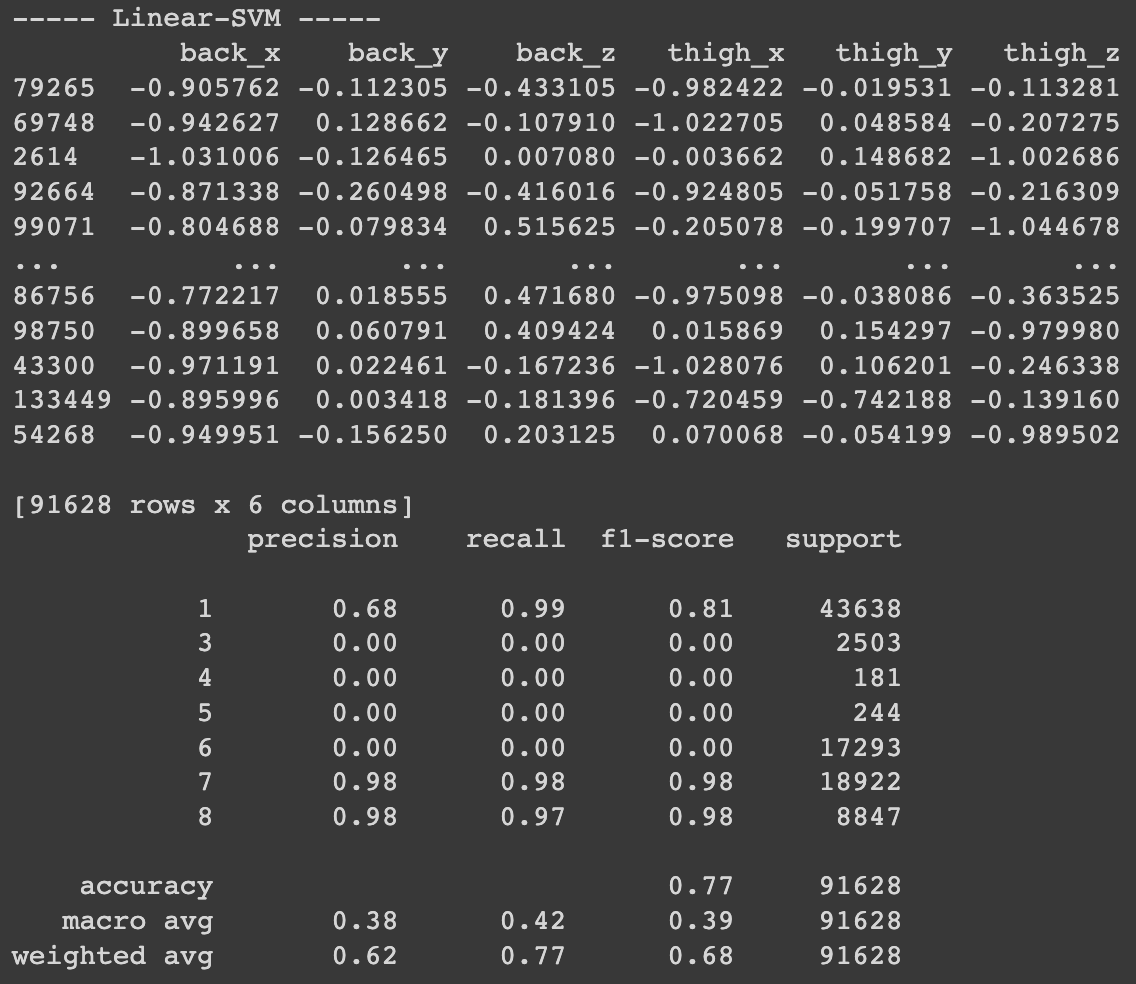
\includegraphics[scale=0.4]{/Users/manuelcardenas/Desktop/Latex/AI/images/r1.png}
        \label{fig:r1}
    \end{figure}
    - \pagebreak

    RBF-SVM and KNN
    \begin{figure}[h]
        \centering
        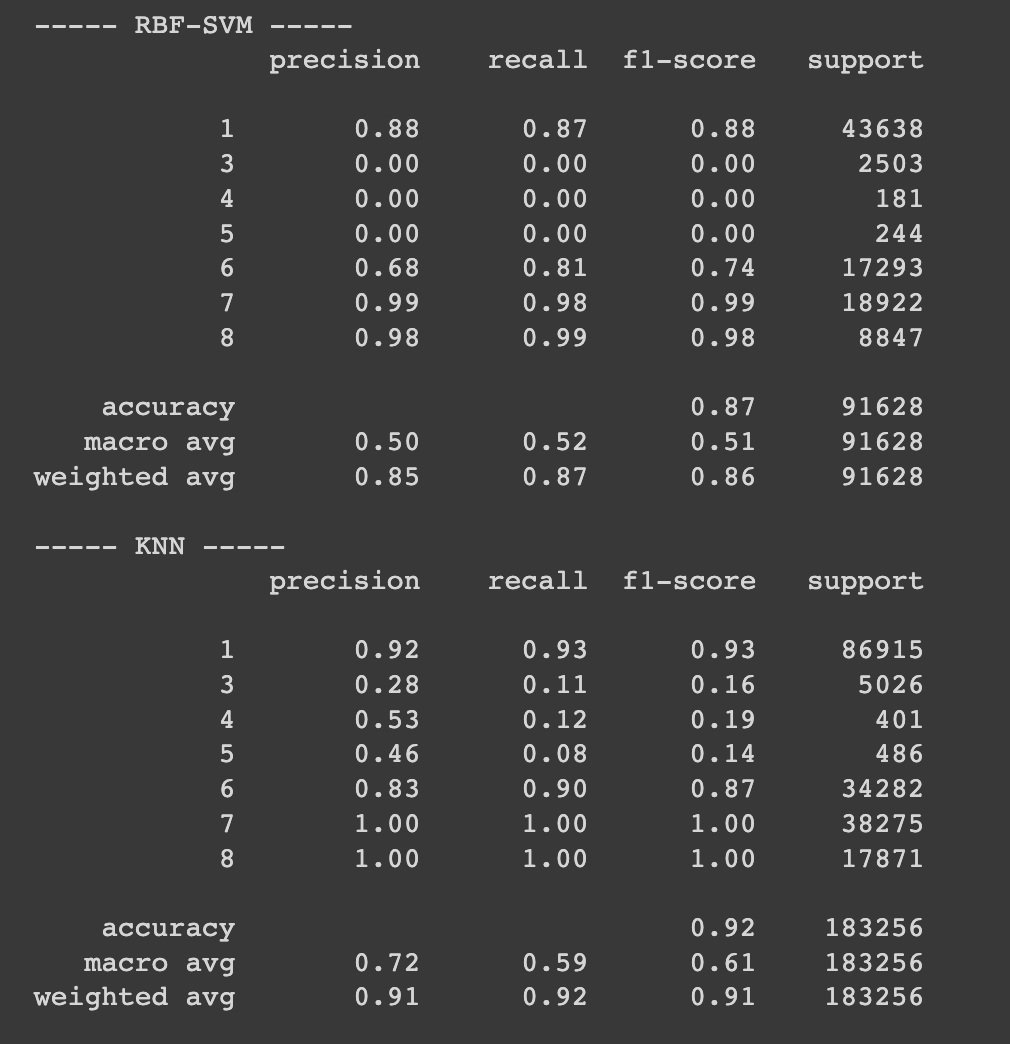
\includegraphics[scale=0.4]{/Users/manuelcardenas/Desktop/Latex/AI/images/r2.png}
        \label{fig:r2}
    \end{figure}
    - \pagebreak

    Decision Tree and Linear Discriminant
    \begin{figure}[h]
        \centering
        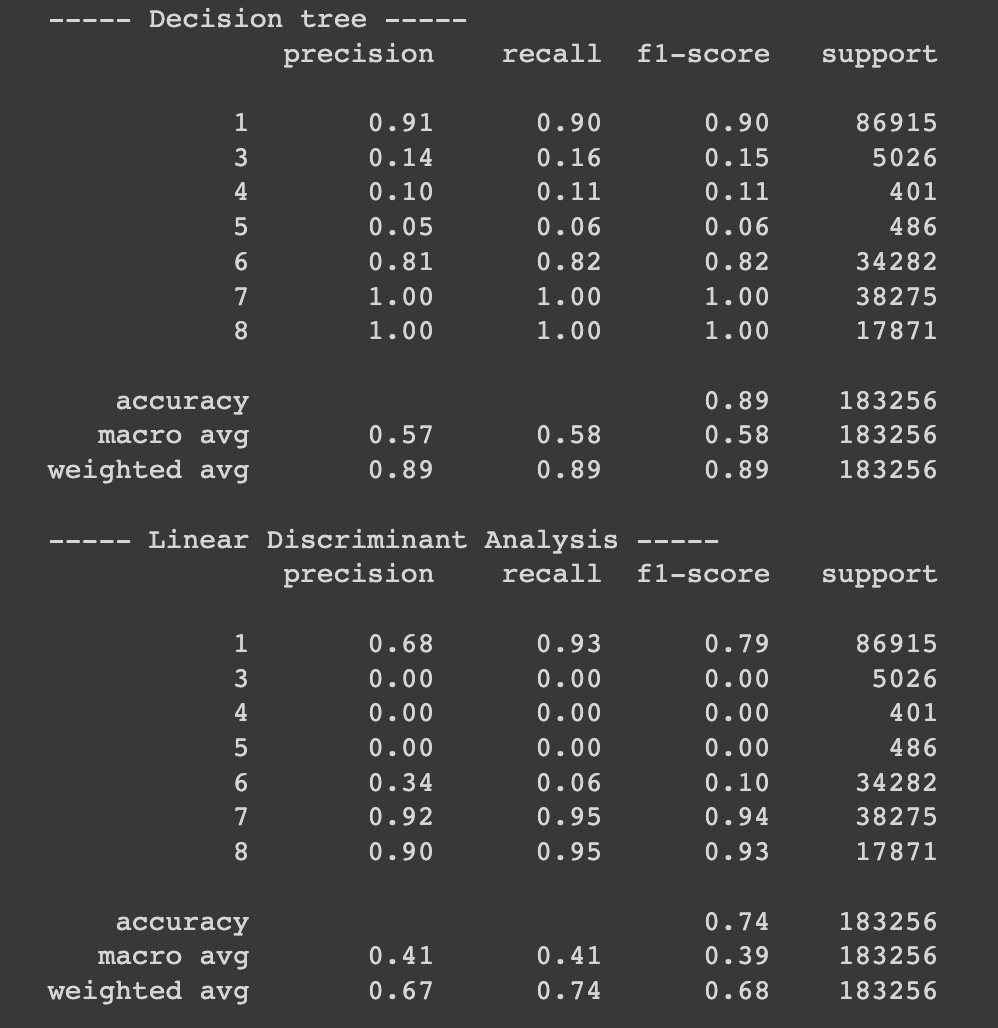
\includegraphics[scale=0.4]{/Users/manuelcardenas/Desktop/Latex/AI/images/r3.png}
        \label{fig:r3}
    \end{figure}
    - \pagebreak

    Random Forest and Gradient Boosting
    \begin{figure}[h]
        \centering
        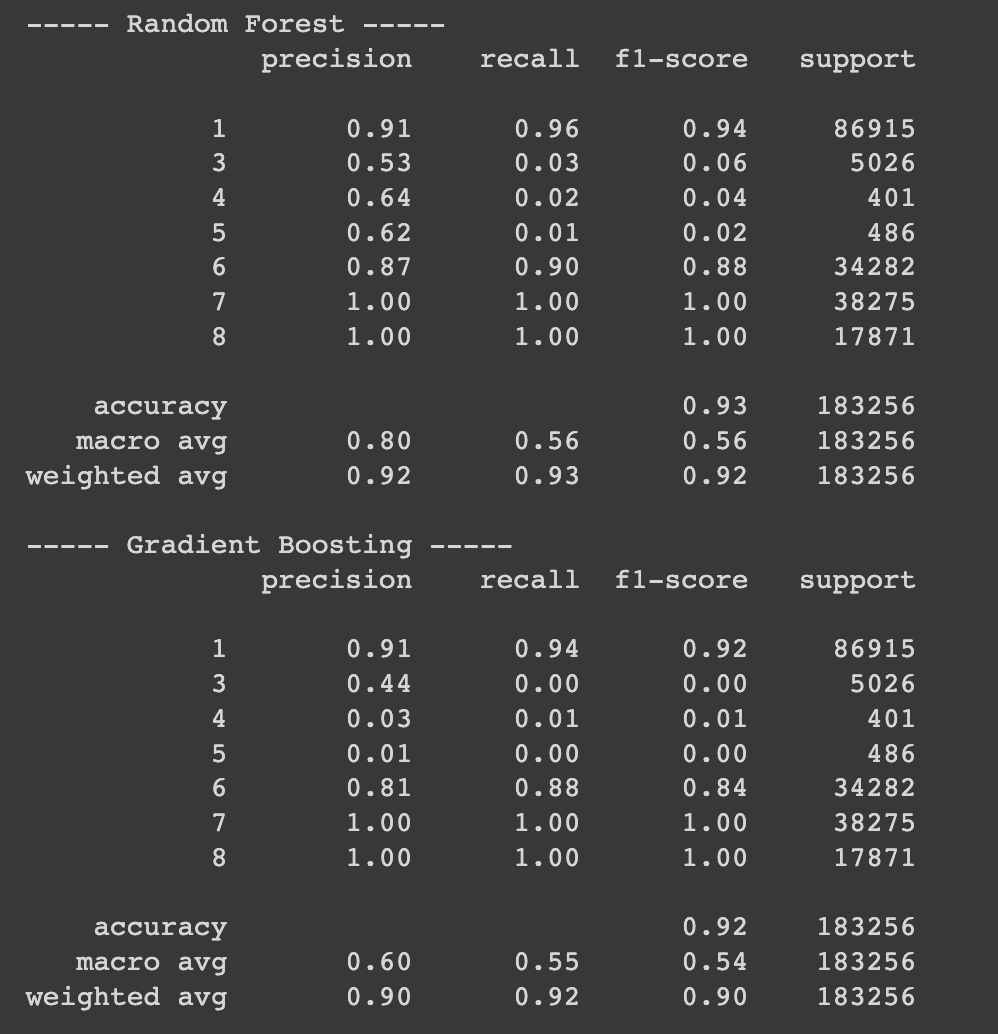
\includegraphics[scale=0.4]{/Users/manuelcardenas/Desktop/Latex/AI/images/r4.png}
        \label{fig:r4}
    \end{figure}
    - \pagebreak

    Polynomial SVM
    \begin{figure}[h]
        \centering
        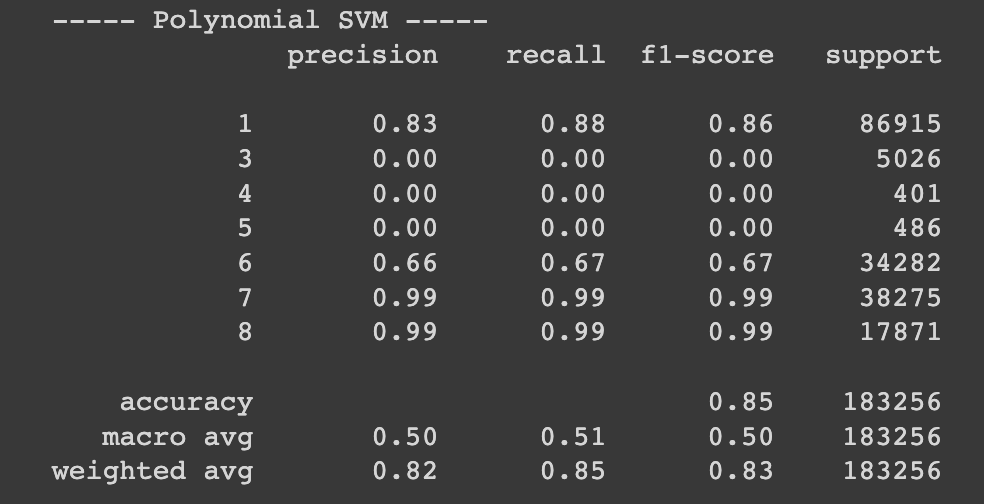
\includegraphics[scale=0.4]{/Users/manuelcardenas/Desktop/Latex/AI/images/r5.png}
        \label{fig:r5}
    \end{figure}

    \subsection{Random Forest and Balanced Random Forest Model}

    Considering the results of all the models, we decided to use two: Random Forest, which gave us the best precisión, 
    and Balanced Random Forest, which displayed the highest recall from all the models. The code focuses on classification 
    using these two methods. It begins by sampling the dataset and extracting features and labels. It then trains and evaluates 
    a Random Forest classifier and a Balanced Random Forest classifier using 3-fold stratified cross-validation, presenting 
    classification reports for both. Afterwards, it creates an ensemble using a Voting Classifier that combines both classifiers 
    and evaluates the ensemble's performance using the same cross-validation approach, generating a classification report. 
    The goal is to compare the individual and combined performances of Random Forest and Balanced Random Forest, exploring 
    the potential benefits of an ensemble approach for classification tasks.\pagebreak
    Random Forest
    \begin{figure}[h]
        \centering
        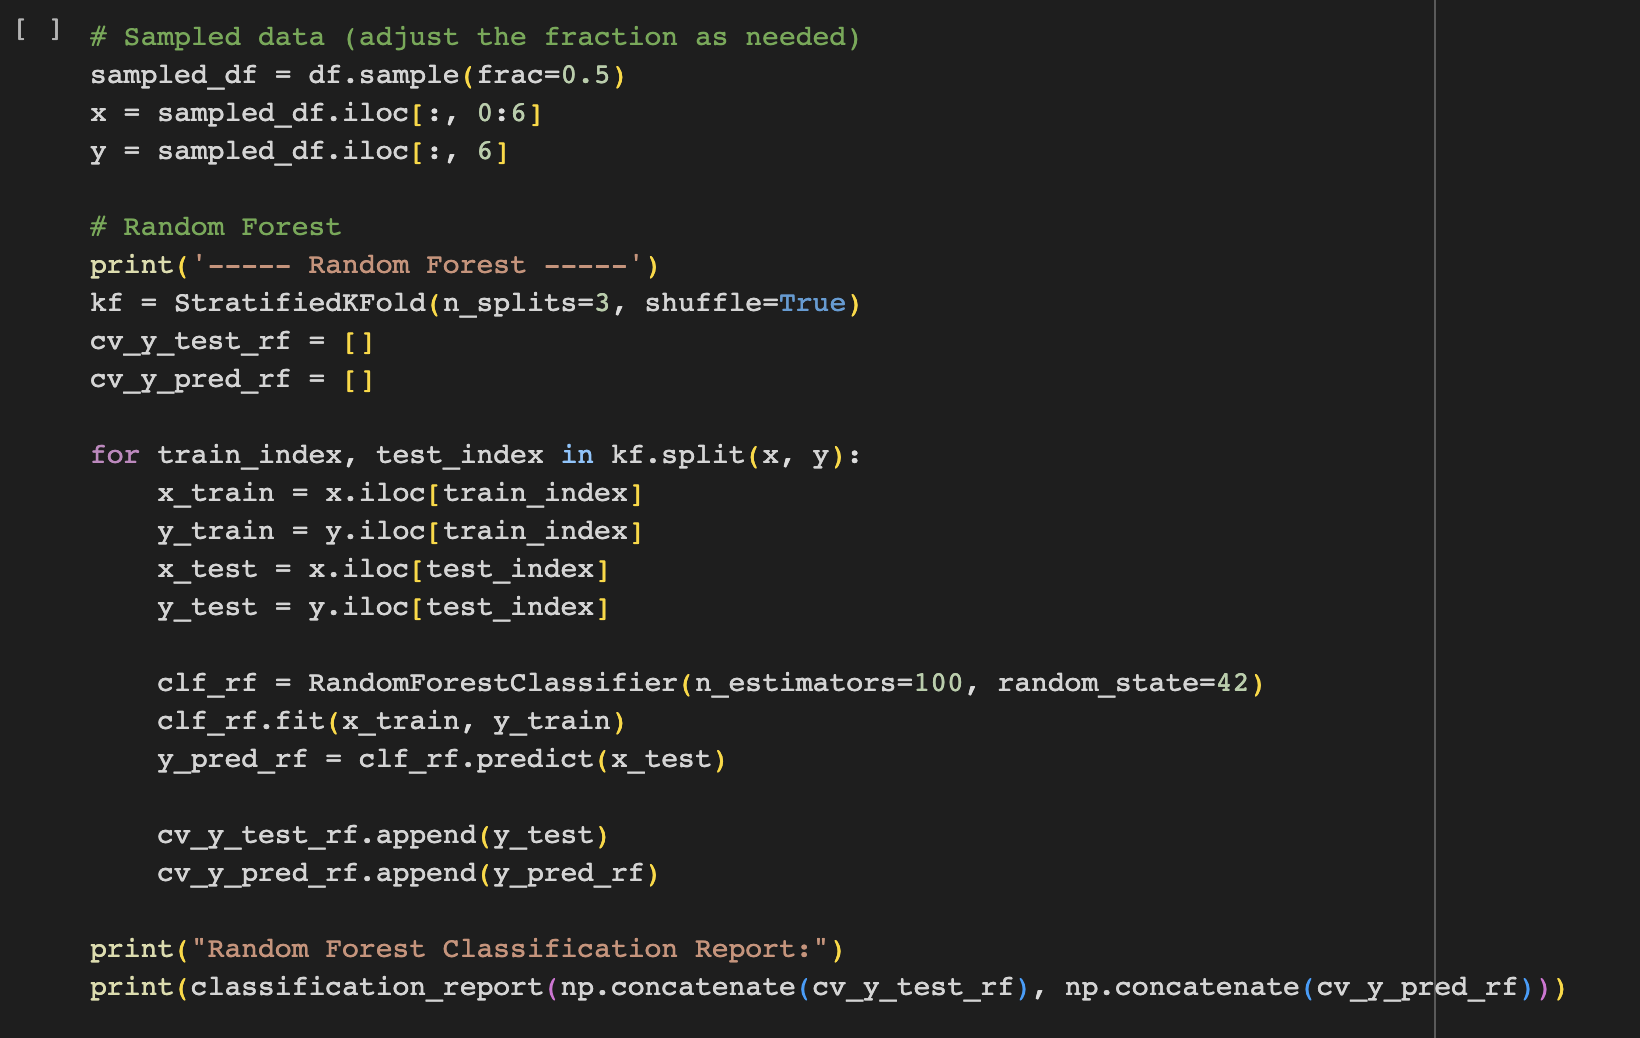
\includegraphics[scale=0.4]{/Users/manuelcardenas/Desktop/Latex/AI/images/rf1.png}
        \label{fig:rf1}
    \end{figure}
    - \pagebreak

    Balanced Random Forest
    \begin{figure}[h]
        \centering
        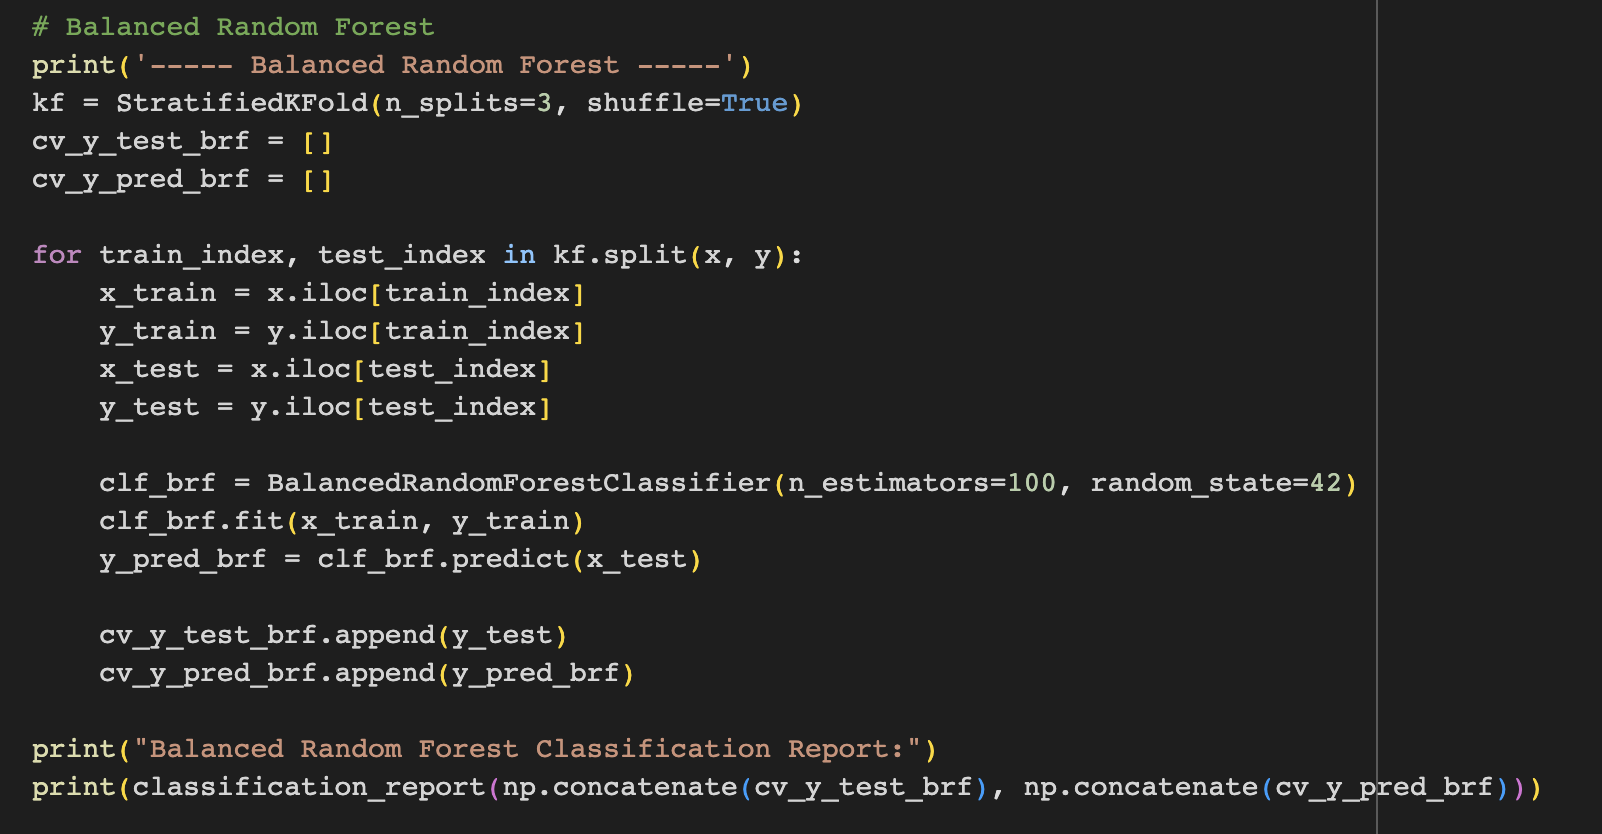
\includegraphics[scale=0.4]{/Users/manuelcardenas/Desktop/Latex/AI/images/rf2.png}
        \label{fig:rf2}
    \end{figure}
    - \pagebreak

    Ensemble both classifiers
    \begin{figure}[h]
        \centering
        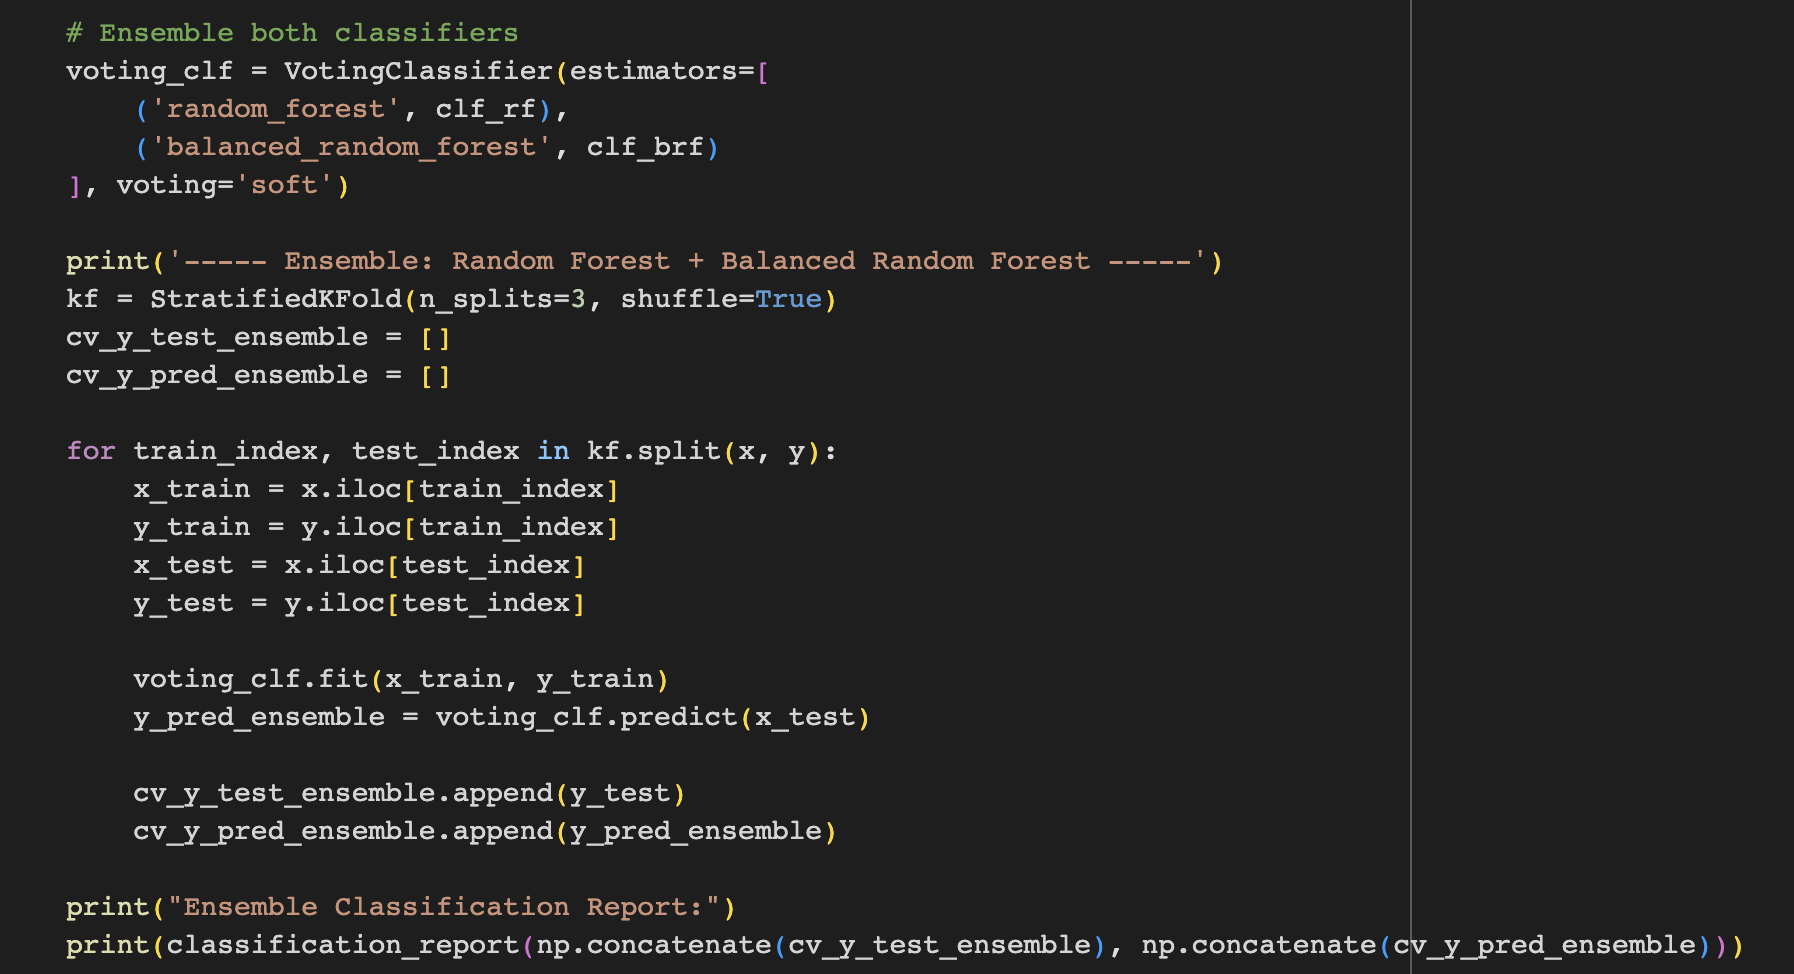
\includegraphics[scale=0.4]{/Users/manuelcardenas/Desktop/Latex/AI/images/rf3.png}
        \label{fig:rf3}
    \end{figure}
    
    As we can see both methods individually have great results for precision and recall respectively. 
    By ensembling a method with both we get a new method in the middle. It doesn't have the precision from the Random Forest nor the recall of the Balanced Random Forest, instead it has an in between.\pagebreak

    Random Forest and Balanced Random Forest Results
    \begin{figure}[h]
        \centering
        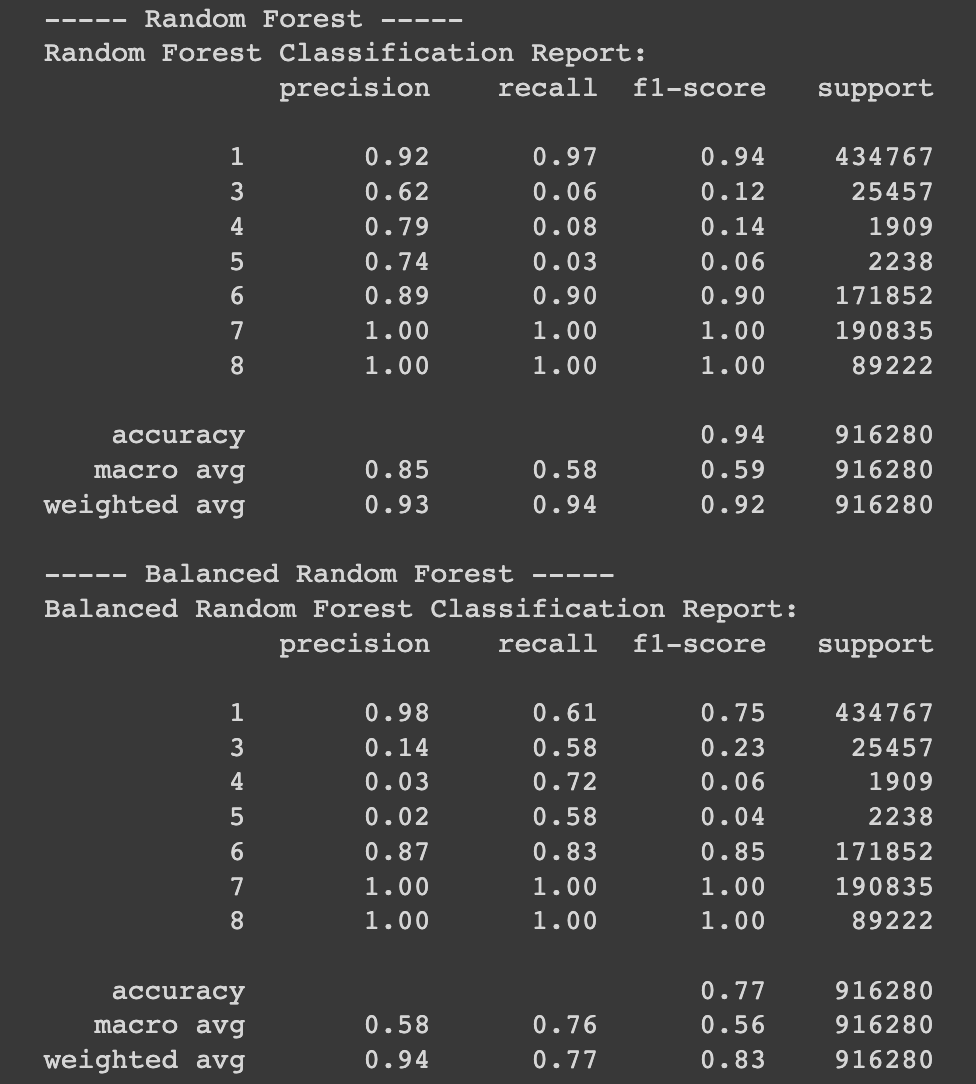
\includegraphics[scale=0.4]{/Users/manuelcardenas/Desktop/Latex/AI/images/rf4.png}
        \label{fig:rf4}
    \end{figure}
    - \pagebreak

    Random Forest + Balanced Random Forest Results
    \begin{figure}[h]
        \centering
        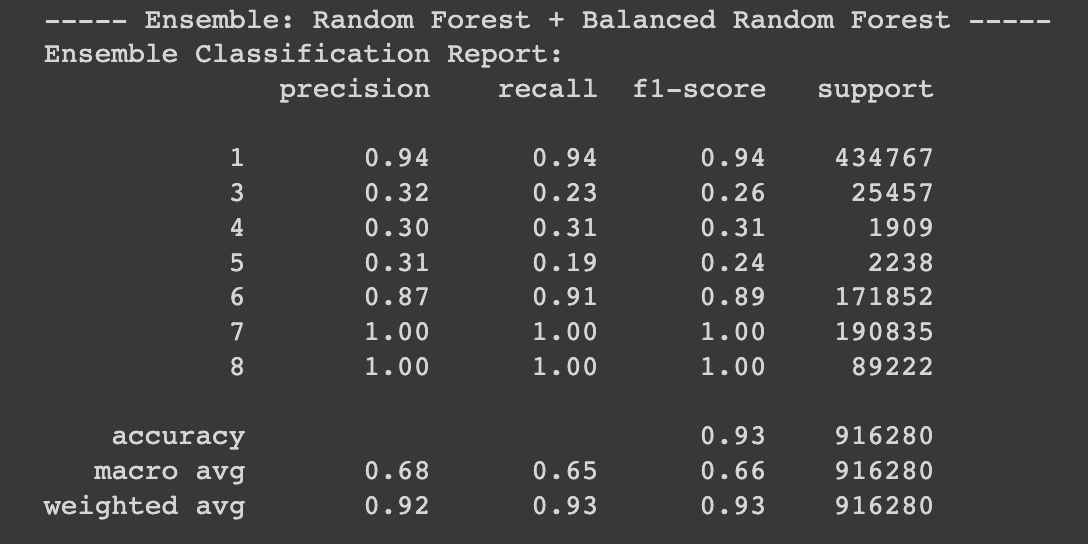
\includegraphics[scale=0.4]{/Users/manuelcardenas/Desktop/Latex/AI/images/rf5.png}
        \label{fig:rf5}
    \end{figure}

    \subsection{Optimal Selection of Hyperparameters}

    Next, we decided to search for the optimal number of hyperparameters. The following code conducts a comprehensive 
    evaluation of the same machine learning classifiers (Random Forest, Balanced Random Forest, and an ensemble of both using 
    a Voting Classifier) just as before. Then the hyperparameters are optimized through randomized search. The ensemble is evaluated 
    using the best hyperparameters and another classification report is generated. This process enables a thorough assessment 
    of individual classifiers and an ensemble, demonstrating how hyperparameter tuning can enhance the performance of an ensemble 
    combining diverse classifiers.\pagebreak
    Random Forest
    \begin{figure}[h]
        \centering
        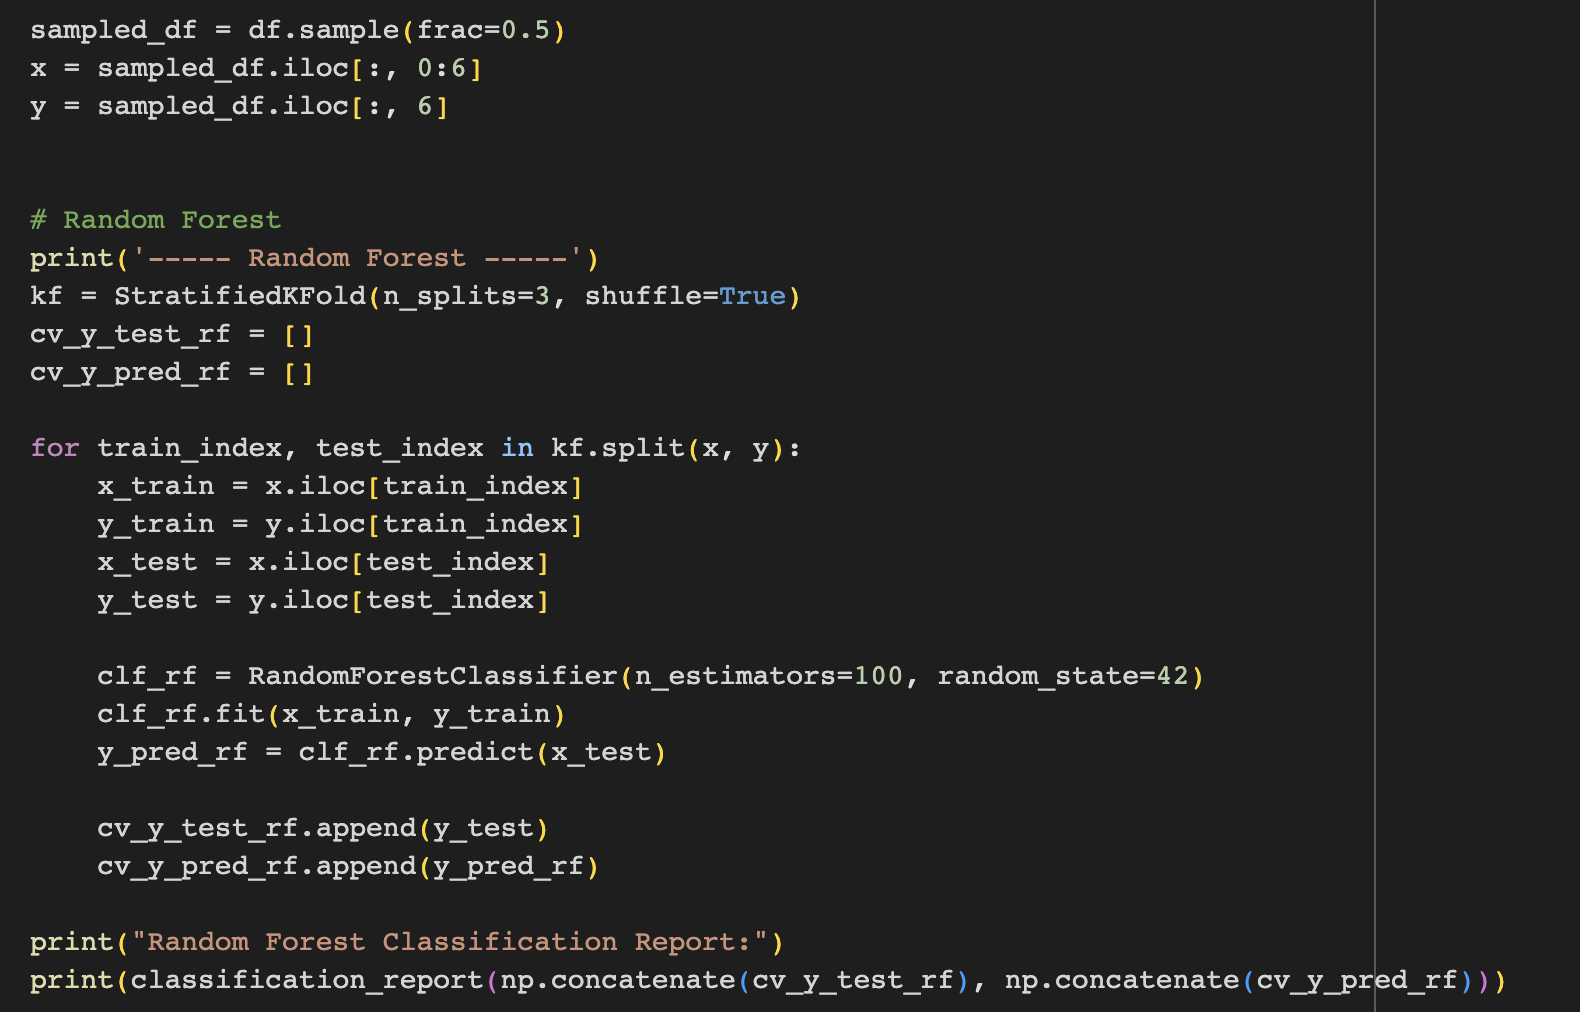
\includegraphics[scale=0.4]{/Users/manuelcardenas/Desktop/Latex/AI/images/h1.png}
        \label{fig:h1}
    \end{figure}
    - \pagebreak

    Balanced Random Forest
    \begin{figure}[h]
        \centering
        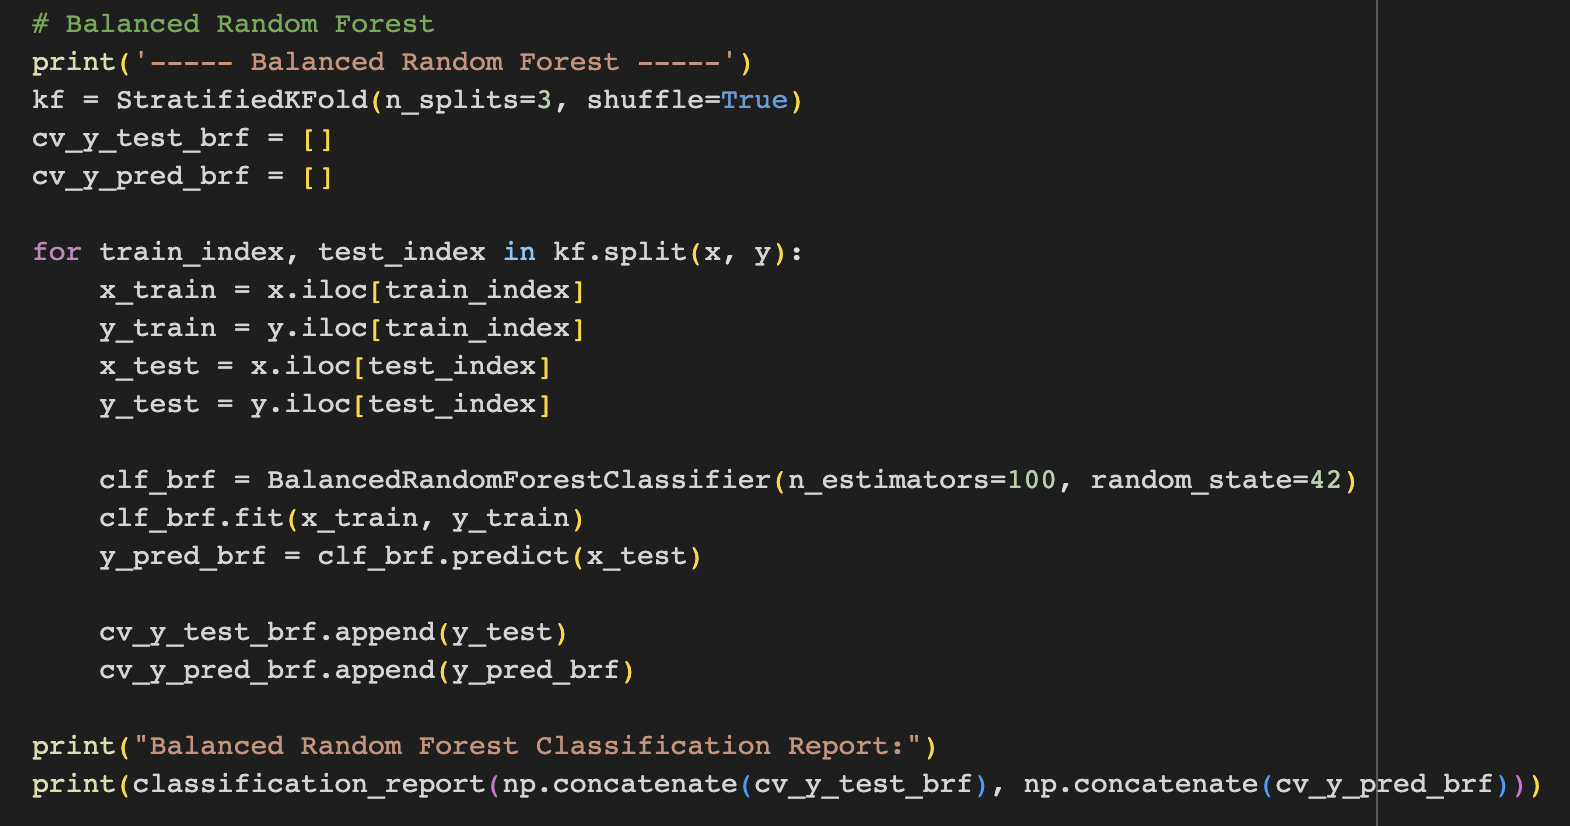
\includegraphics[scale=0.4]{/Users/manuelcardenas/Desktop/Latex/AI/images/h2.png}
        \label{fig:h2}
    \end{figure}
    - \pagebreak

    Hyperparameters part 1
    \begin{figure}[h]
        \centering
        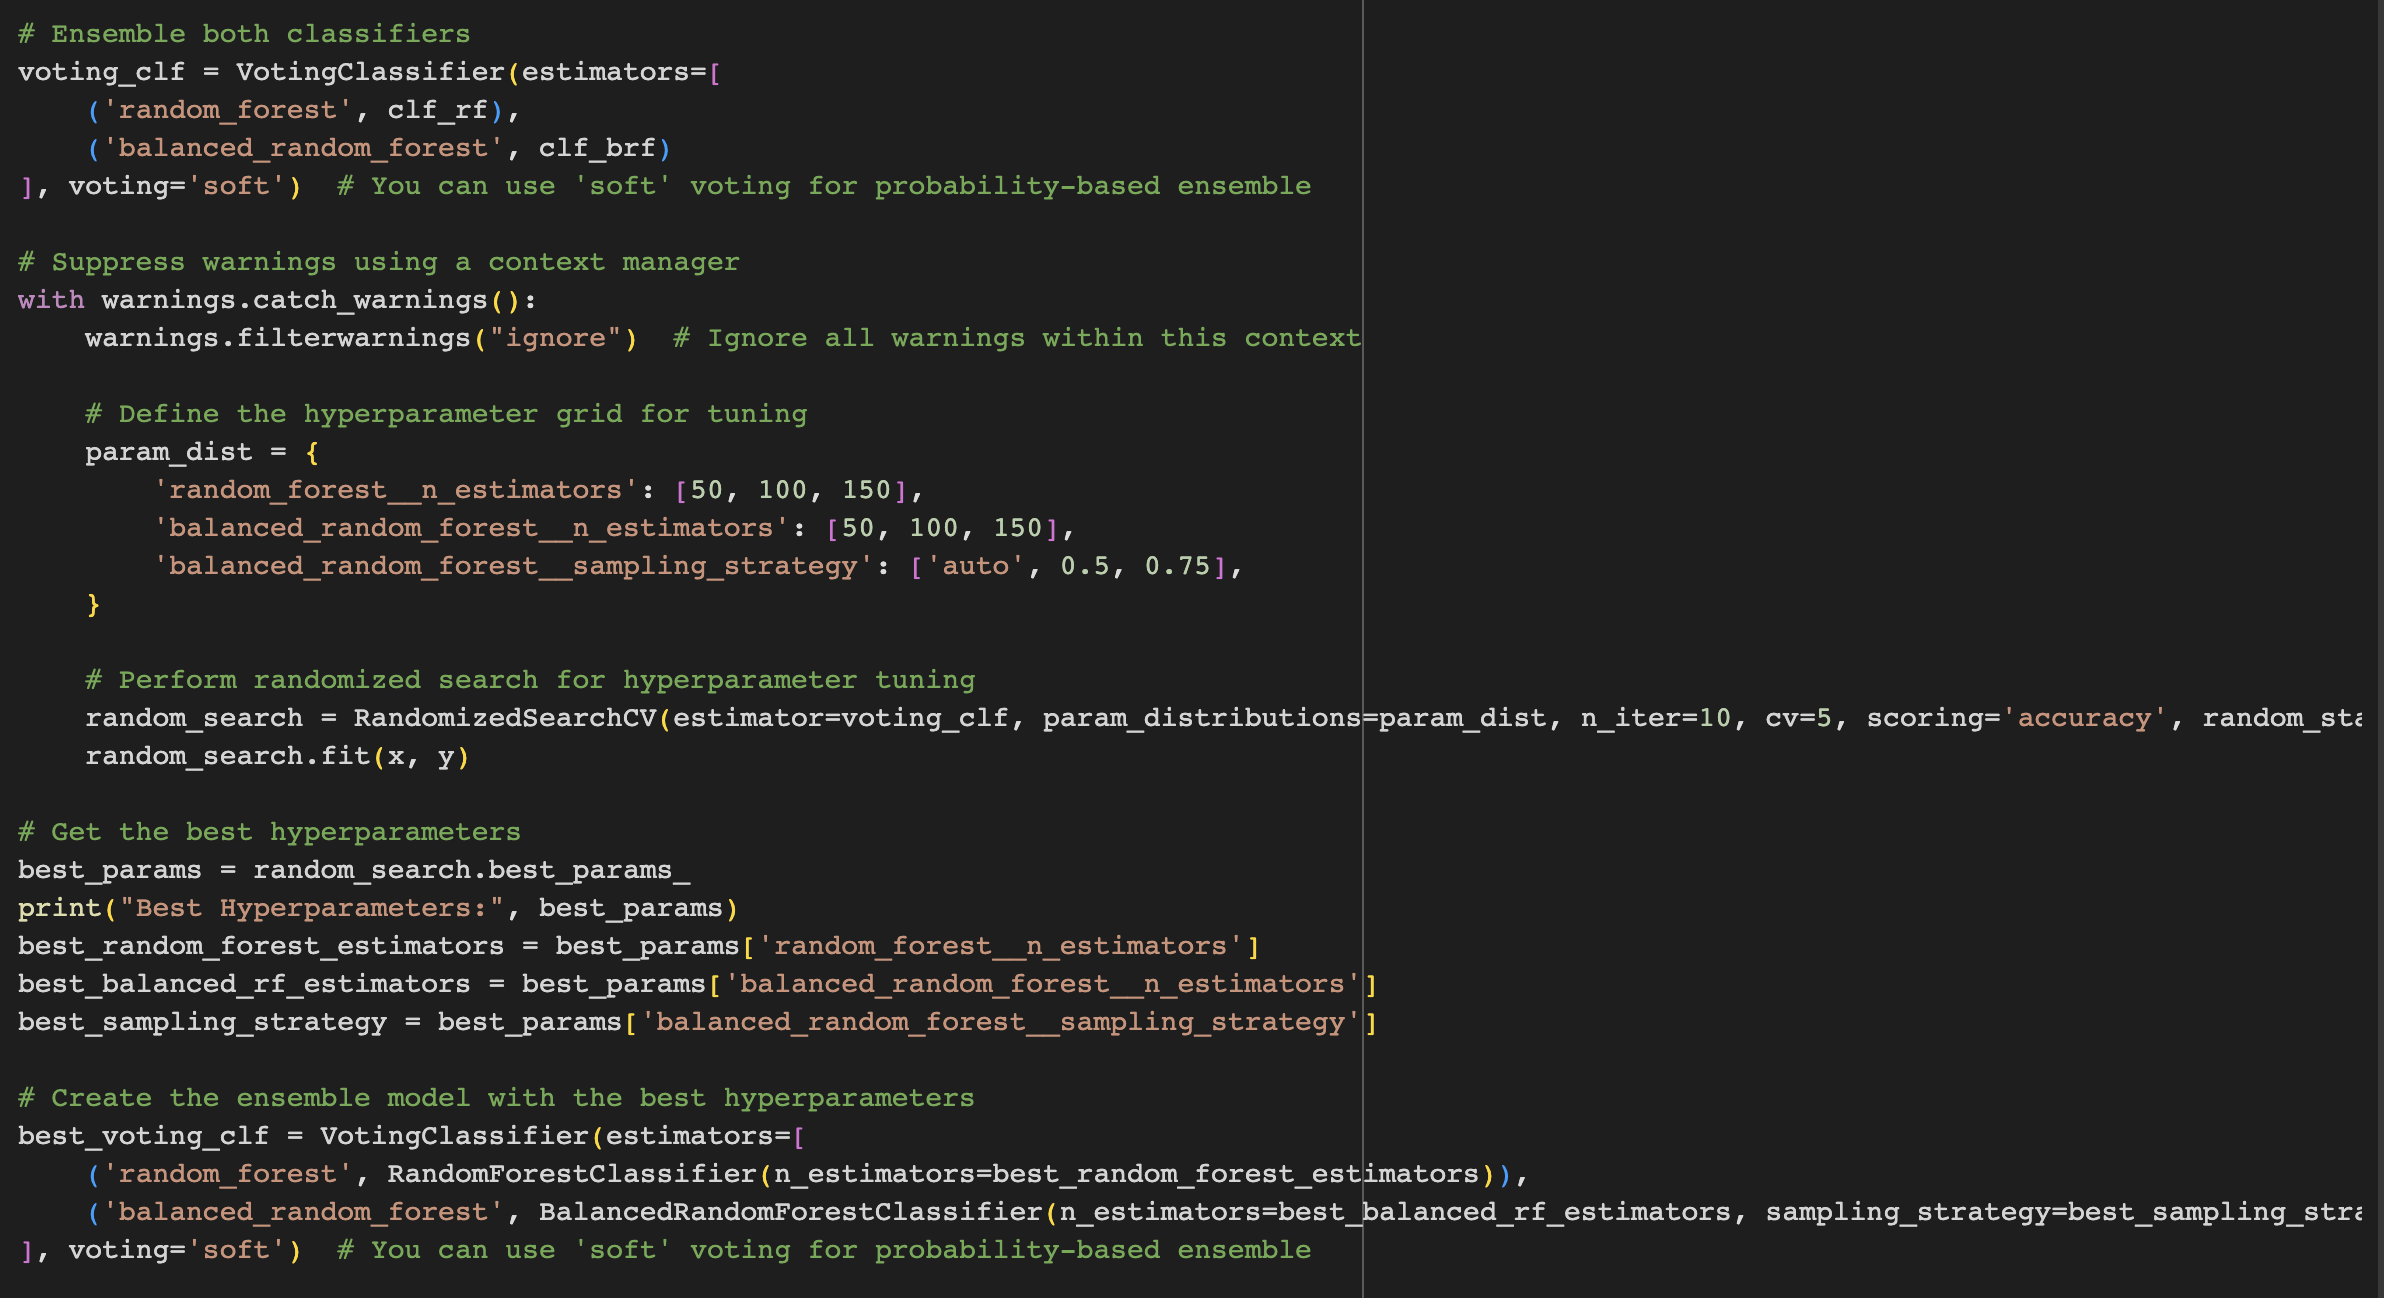
\includegraphics[scale=0.4]{/Users/manuelcardenas/Desktop/Latex/AI/images/h3.png}
        \label{fig:h3}
    \end{figure}
    - \pagebreak

    Hyperparameters part 2
    \begin{figure}[h]
        \centering
        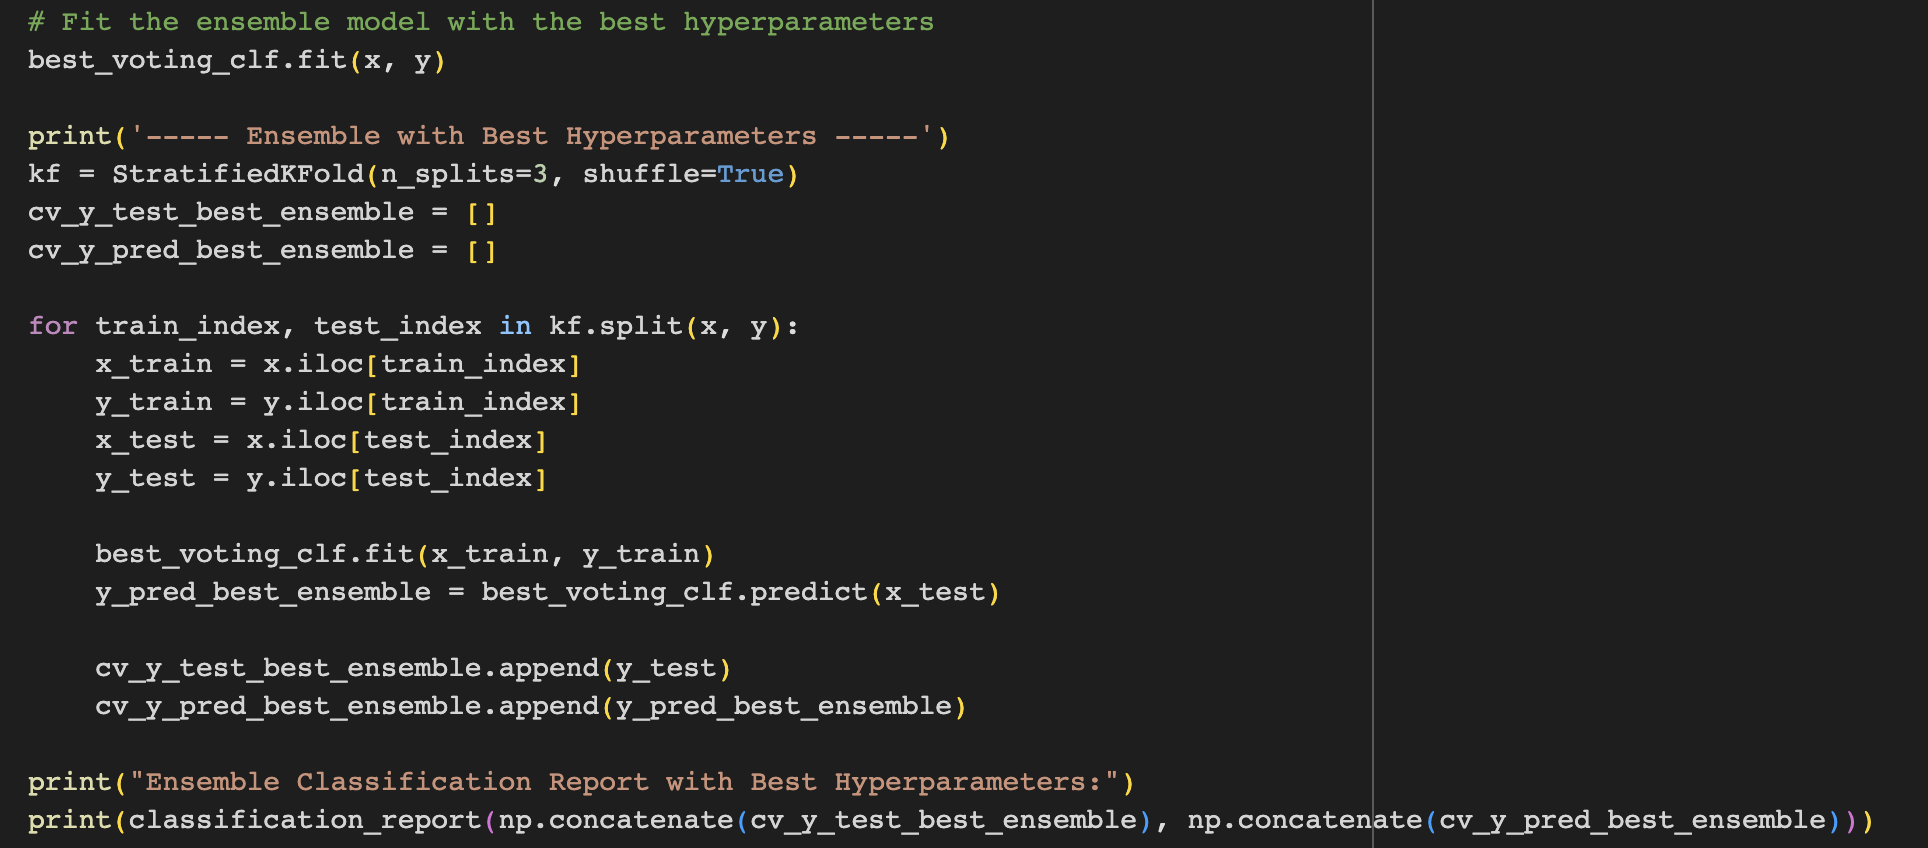
\includegraphics[scale=0.4]{/Users/manuelcardenas/Desktop/Latex/AI/images/h4.png}
        \label{fig:h4}
    \end{figure}
    
    By getting the optimal number of hyperparameter we can now test the model and models results for precision,  recall and f1 \pagebreak

    Random Forest and Balanced Random Forest Results
    \begin{figure}[h]
        \centering
        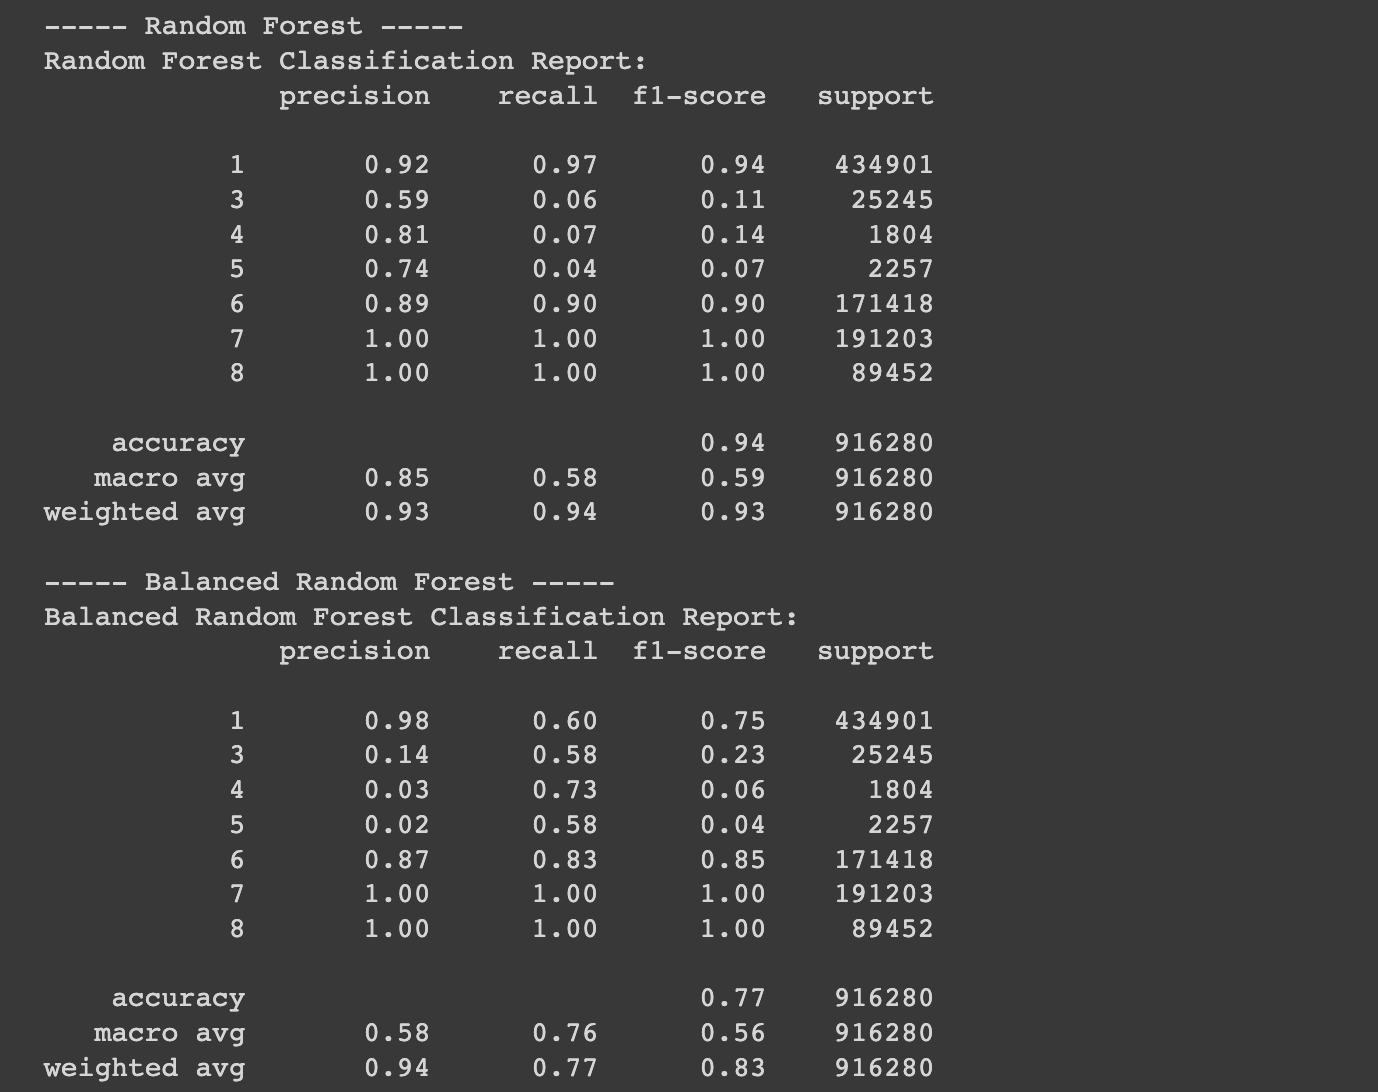
\includegraphics[scale=0.4]{/Users/manuelcardenas/Desktop/Latex/AI/images/h5.png}
        \label{fig:h5}
    \end{figure}
    - \pagebreak

    Hyperparameters
    \begin{figure}[h]
        \centering
        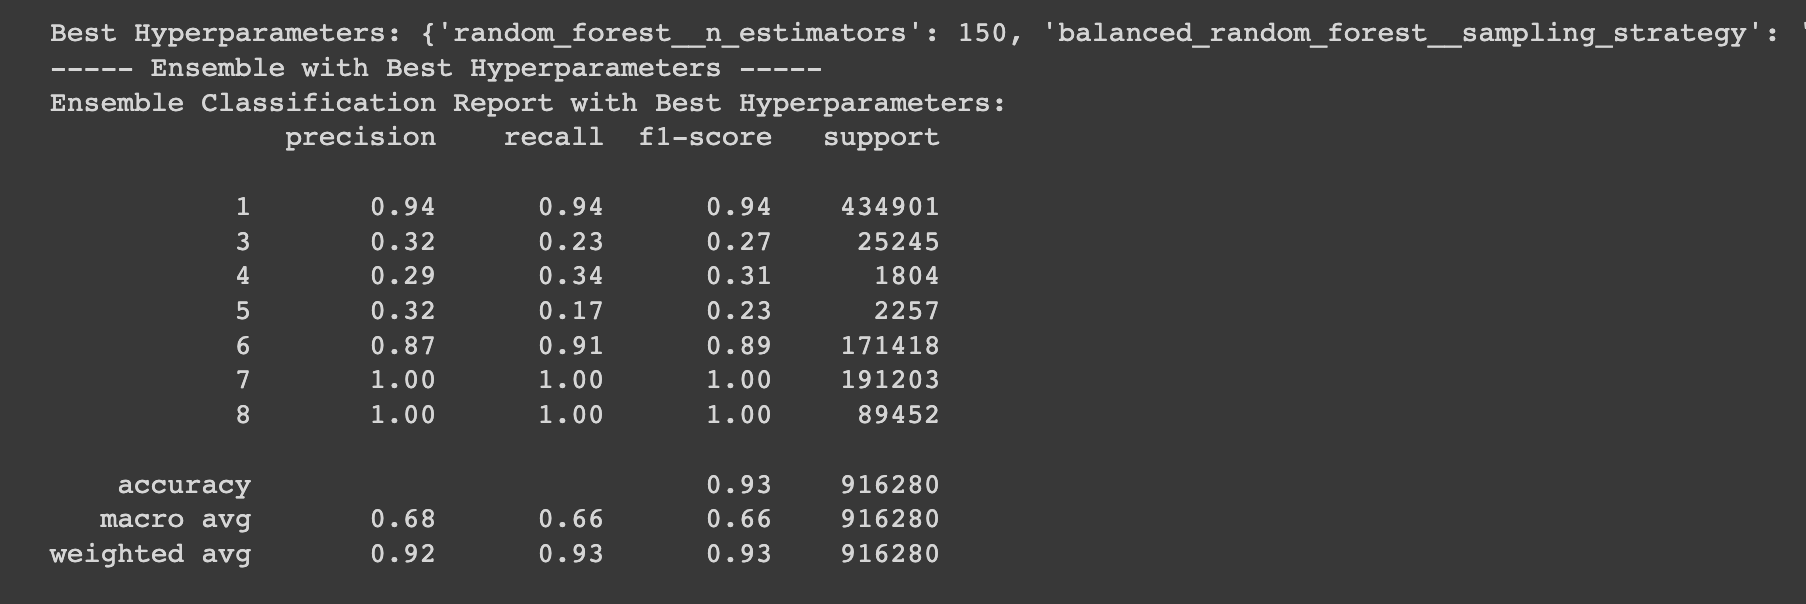
\includegraphics[scale=0.4]{/Users/manuelcardenas/Desktop/Latex/AI/images/h6.png}
        \label{fig:h6}
    \end{figure}

    \subsection{Model tuning with hyperparameters}

    Lastly, we adjust the method with the hyperparameter from the previous example. This should allow for the optimization
     of the model's performance metrics like accuracy, precision, recall, and F1-score.\pagebreak
     Model with Hyperparameters
     \begin{figure}[h]
         \centering
         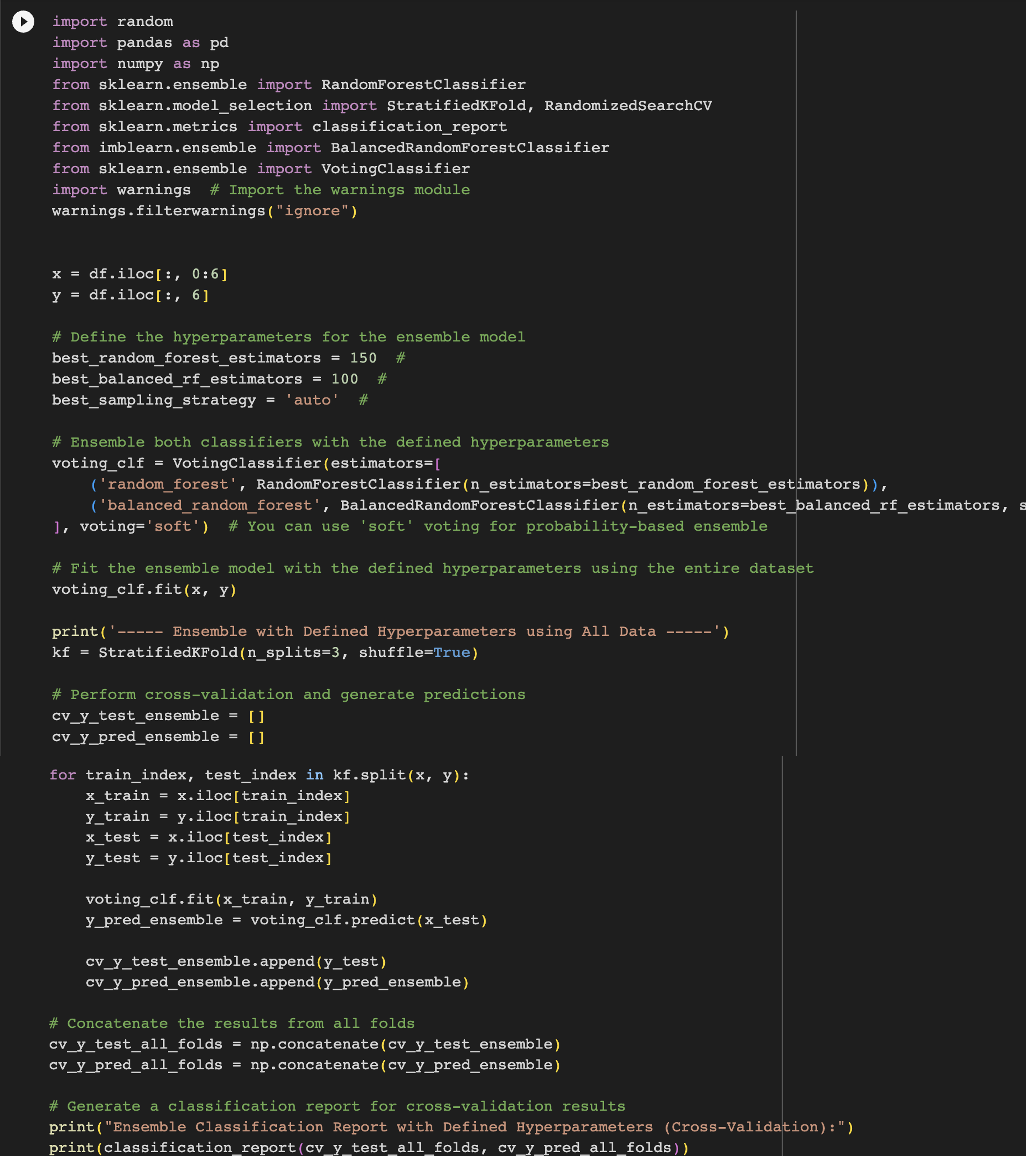
\includegraphics[scale=0.4]{/Users/manuelcardenas/Desktop/Latex/AI/images/hyp1.png}
         \label{fig:hyp1}
     \end{figure}
 
     The result display that the model has improved greatly from  its initial predictions.
      Now, the precision has gotten exponentially better in the most unbalanced labels while also improving on the models recall. 
      This means that the models prediction will increase and it's a more oprimize and funcional model\pagebreak
      Results
     \begin{figure}[h]
         \centering
         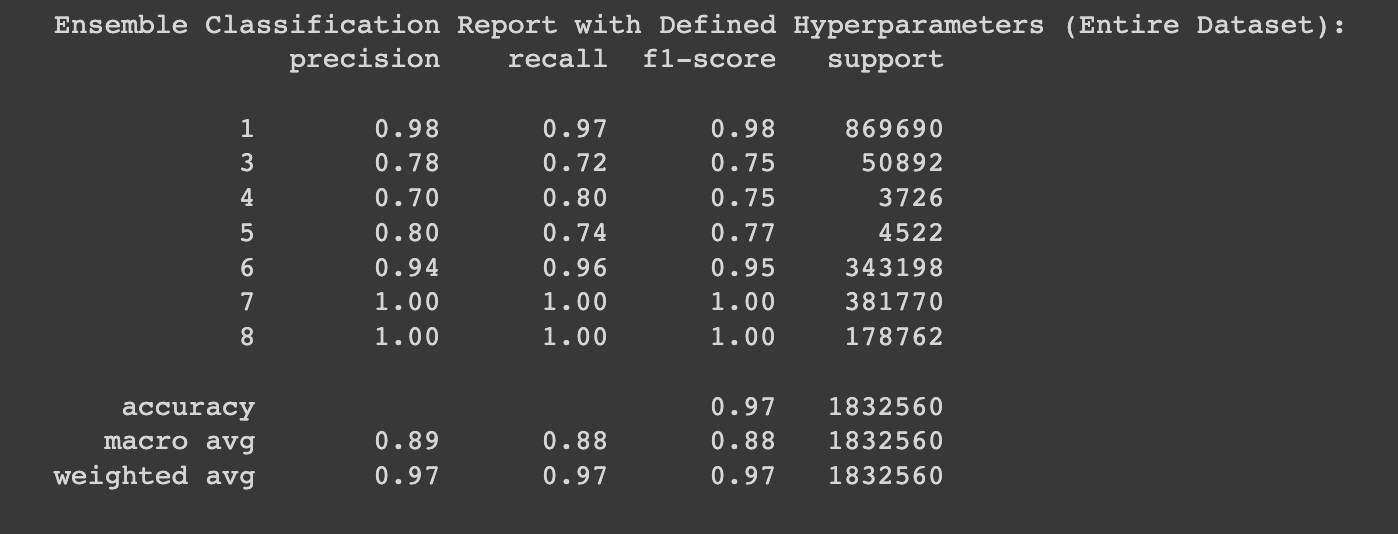
\includegraphics[scale=0.4]{/Users/manuelcardenas/Desktop/Latex/AI/images/hyp2.png}
         \label{fig:hp2}
     \end{figure}


\section{Flask}
     The following code saves the model in a json, so that it can be passed to a Flask 
     server with an interface to run the program and make predictions.
     \begin{figure}[h]
         \centering
         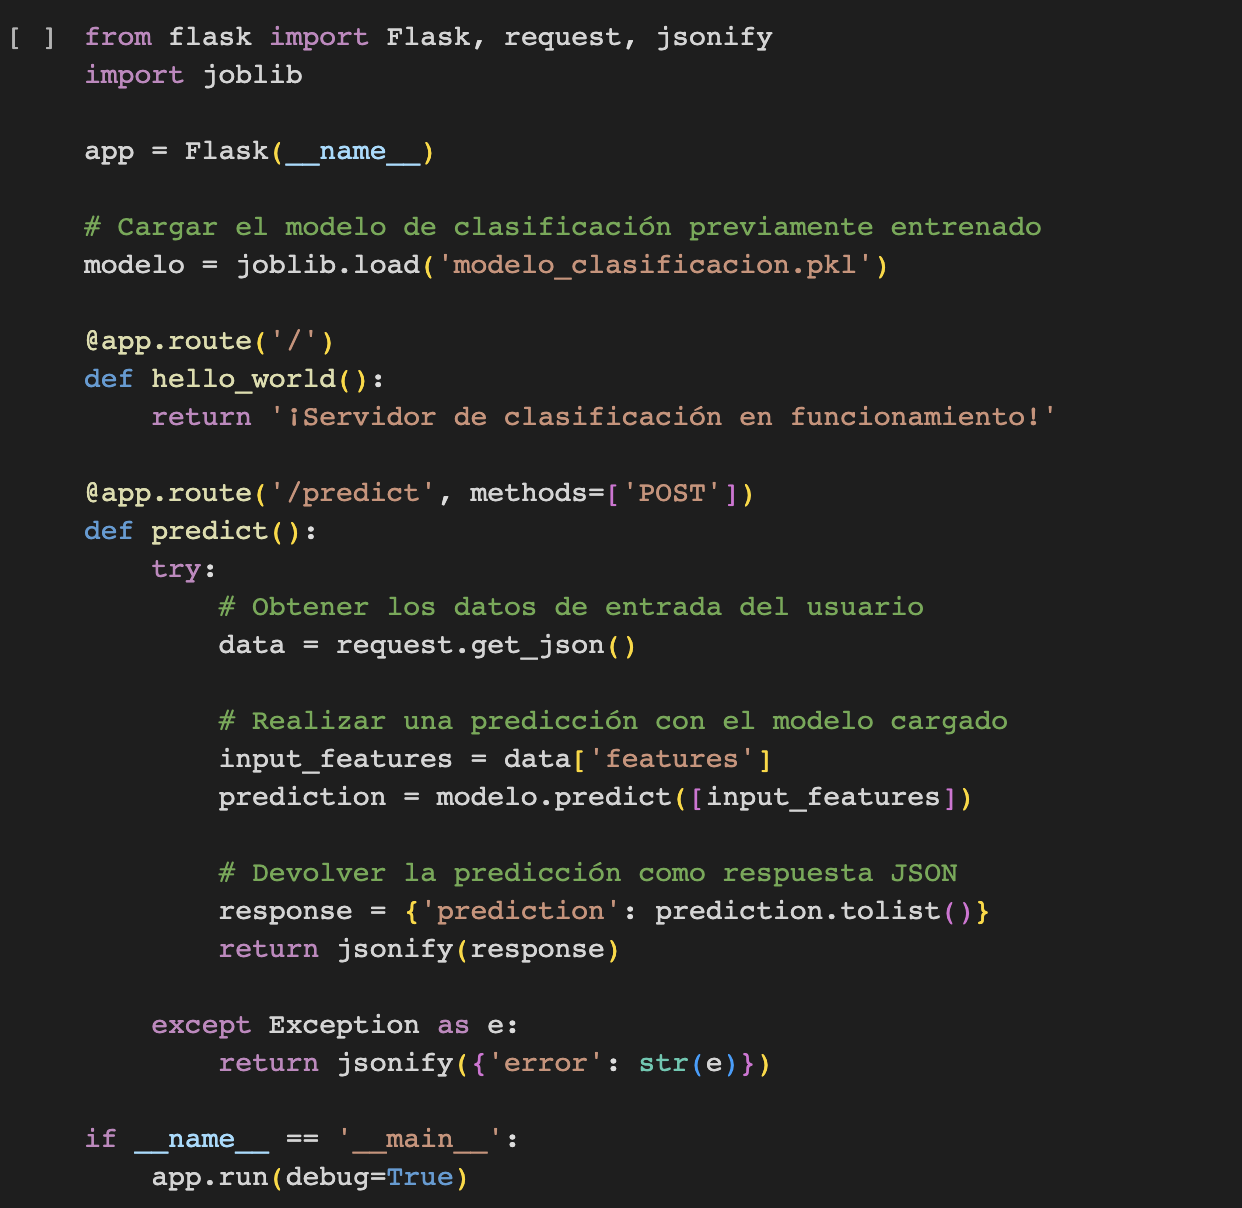
\includegraphics[scale=0.4]{/Users/manuelcardenas/Desktop/Latex/AI/images/f1.png}
         \label{fig:f1}
     \end{figure}

\bibliographystyle{plain}
\bibliography{references}
\end{document}